% +--------------------------------------------------------------------+
% | LaTeX Template                                                     |
% | for K-State Electronic Theses, Dissertations, and Reports          |
% |                                                                    |
% | Comments and guidelines for using the template are shown           |
% | within boxes like this one.                                        |
% |                                                                    |
% | Revised 6/30/06                                                    |
% | 9/14/06: Removed typos                                             |
% +--------------------------------------------------------------------+

% +--------------------------------------------------------------------+
% | Your paper should contain the following sections, except where     |
% | indicated as optional, in the order shown.  Also, all headings     |
% | shown with an asterisk (*) must be centered and in uppercase       |
% | letters:                                                           |
% |                                                                    |
% | Abstract Title Page (doctoral dissertations only)                  |
% | ABSTRACT* (doctoral dissertations only)                            |
% | Title Page                                                         |
% | Copyright Page (Optional - only needed if copyrighting)            |
% | ABSTRACT *                                                         |
% | TABLE OF CONTENTS *                                                |
% | LIST OF FIGURES *                                                  |
% | LIST OF TABLES*                                                    |
% | ACKNOWLEDGMENTS* (Optional)                                        |
% | DEDICATION * (Optional)                                            |
% | PREFACE * (Optional)                                               |
% | Individual Chapters                                                |
% | References and/or bibliography                                     |
% | Appendices (as needed)                                             |
% +--------------------------------------------------------------------+

% +--------------------------------------------------------------------+
% | The LaTex keyword \documentclass selects a particular class to     |
% | associate with the document.  The current documentclass            |
% | {class_diss} generates a Table of Contents that has leading dots   |
% | only on chapter subheadings.  If you prefer a Table of Contents    |
% | that has leading dots for all entries, replace {class_diss}        |
% | with {Mydiss} in the command below.                                |
% |                                                                    |
% +--------------------------------------------------------------------+

\documentclass[final, 12pt,oneside]{class_diss}

% +--------------------------------------------------------------------+
% | The following command sets the bibliography style to American
% | Institute of Physics (AIP).  Other styles are available in the
% | styles directory.  To use a different style, replace "aip" with
% | the filename of the style you want to use.
% +--------------------------------------------------------------------+

\bibliographystyle{styles/plain}

\usepackage[utf8]{inputenc}
\usepackage[T1]{fontenc}
\usepackage[spanish]{babel}
% +--------------------------------------------------------------------+
% | Now, we add in all external packages that we will use throughout   |
% | the document.  You can add other packages as needed.
% +--------------------------------------------------------------------+

%\usepackage{     caption2} % Customize captions a bit more
\usepackage{      amsmath} % American Mathematics Society standards
%\usepackage{      wrapfig} % Wraps text around a figure or table
\usepackage{     graphicx} % Extended graphics package.
%\usepackage{     fancyhdr} % Efficiently handles headers and footers
%\usepackage{       braket} % Bra-Ket notation package
%\usepackage{     mathrsfs} % Specialized Math fonts (Hamiltonian, etc.)
%\usepackage{boxedminipage} % Boxed text can be produced
%\usepackage{     setspace} % Controls line spacing via \begin{space}

\usepackage{amsxtra}
\usepackage{amssymb}
\usepackage{amsthm}
\usepackage{latexsym}
\usepackage[official]{eurosym}


% +--------------------------------------------------------------------+
% | The color package allows one to select colors for hyperlinking     |
% | (see below).                                                       |
% +--------------------------------------------------------------------+

\usepackage[usenames]{color}

% +--------------------------------------------------------------------+
% | Colors defined for use with this template.                         |
% +--------------------------------------------------------------------+

\definecolor{  Pink}{rgb}{1.0, 0.5, 0.5}
\definecolor{Maroon}{rgb}{0.8, 0.0, 0.0}

% +--------------------------------------------------------------------+
% | In the commands below, we use the 'natbib' package, and specify    |
% | the 'sort&compress' option, which condenses                        |
% | citations from (1,2,3,5,9,10,11) to (1-3,5,9-11).  The 'bibpunct'  |
% | option selects various parameters for how the citation will be     |
% | displayed.  In this case, only the comma (separation between       |
% | citations) and the 's' (superscript) arguments are chosen.  The    |
% | other curly braces deal with how to 'wrap' the citation (using     |
% | parentheses, brackets, etc.) and are not needed for the chosen     |
% | style.                                                             |
% +--------------------------------------------------------------------+

\usepackage[sort&compress]{natbib}
\bibpunct{}{}{,}{s}{}{}
\usepackage{hypernat}

% +--------------------------------------------------------------------+
% | Lastly, the hyperref package allows one to hyperlink cross-        |
% | references and figures in a LaTeX document.                        |
% +--------------------------------------------------------------------+

\usepackage[pdftex, plainpages=false, pdfpagelabels]{hyperref}

\hypersetup{
    linktocpage=true,
    colorlinks=true,
    bookmarks=true,
    citecolor=blue,
    urlcolor=red,
    linkcolor=Maroon,
    citebordercolor={1 0 0},
    urlbordercolor={1 0 0},
    linkbordercolor={.7 .8 .8},
    breaklinks=true,
    pdfpagelabels=true,
    }

% +--------------------------------------------------------------------+
% | Page margins are set on 1 inch on all sides.                       |
% +--------------------------------------------------------------------+

\topmargin      = -0.56in
\textheight     =  8.60in
\textwidth      =  6.46in
\oddsidemargin  =  0.02in

% +--------------------------------------------------------------------+
% | The document finally begins here.                                  |
% +--------------------------------------------------------------------+

\begin{document}


  \setcounter{page}{-1}


% +--------------------------------------------------------------------+
% | Title Page -- Required for both Doctoral and Masters Students
% +--------------------------------------------------------------------+

% +--------------------------------------------------------------------+
% | Title Page
% +--------------------------------------------------------------------+

\newpage

% +--------------------------------------------------------------------+
% | This page should not contain a page number.  We use the
% | \thispagestyle[empty] command below to suppress page numbers
% | and other style elements.
% +--------------------------------------------------------------------+

\thispagestyle{empty}

% +--------------------------------------------------------------------+
% | The Title page begins here.
% +--------------------------------------------------------------------+

\begin{center}

   \vspace{1cm}

% +--------------------------------------------------------------------+
% | On the line below, replace "ENTER YOUR TITLE" with the title of
% | your ETDR.  Use all CAPITAL LETTERS.
% +--------------------------------------------------------------------+

   {\Large ACCELBIKE}\\

   \vspace{0.5cm}



   \vspace{0.5cm}



   {\large RODRIGO CLAUDIO MIGUEZ REIN}\\
   {\large DAVID MUÑOZ LORENZO}\\
   {\large ALEXIS VIZCAYA HERVELLA}\\

   \vspace{0.5cm}




   GRADO EN INGENIERÍA DEL SOFTWARE. FACULTAD DE INFORMÁTICA\\
   UNIVERSIDAD COMPLUTENSE DE MADRID \\


   \vspace{0.65cm}
   \rule{2in}{0.5pt}\\
   \vspace{0.85cm}

  
\includegraphics[height=2.5in]{figures/escudo.jpg}
  

%+-- Escribe el nombre de tu asignatura de fin de master (Ingeniería de computadores,....)
   \vspace{0.5cm}
Trabajo Fin Grado en Ingeniería del Software

   \vspace{0.5cm}





% +--------------------------------------------------------------------+
%  Fecha 
% +--------------------------------------------------------------------+

  17 de Junio de 2016\\
   \vspace{1cm}

\end{center}

{\raggedleft
Directores:\\
   \vspace{ 1cm}
José Ignacio Gómez Pérez\\
Luis Piñuel Moreno\\
}


% +--------------------------------------------------------------------+
% | Use the section below if you have co-major professors.
% +--------------------------------------------------------------------+

%\begin{flushleft}
%   \hspace{10cm}Approved by:\\
%   \vspace{ 1cm}
%   \hspace{10cm}Co-Major Professor\\
%   \hspace{10cm}Enter Your Co-Major Professor's Name\\
%   \vspace{.5cm}
%   \hspace{10cm}Co-Major Professor\\
%   \hspace{10cm}Enter Your Co-Major Professor's Name\\
%\end{flushleft}

   \pdfbookmark[0]{Portada}{PDFPortadaPage}

% +--------------------------------------------------------------------+
% | Autorizacion Page -- Required for both Doctoral and Masters Students
% +--------------------------------------------------------------------+

% +--------------------------------------------------------------------+
% | Copyright Page
% +--------------------------------------------------------------------+

\newpage

\thispagestyle{empty}

\begin{center}

{\bf \Huge Autorización de difusión}

\vspace{1cm}

% +--------------------------------------------------------------------+
% | On the line below, replace "Enter Your Name" with your name
% | Use the same form of your name as it appears on your title page.
% | Use mixed case, for example, Lori Goetsch.
% +--------------------------------------------------------------------+

   \large Autor\\

   \vspace{0.5cm}

% +--------------------------------------------------------------------+
% | On the line below, replace Fecha
% |
% +--------------------------------------------------------------------+

   Fecha\\

   \vspace{0.5cm}
   \end{center}
   
El/la abajo firmante, matriculado/a en el Máster en Investigación en Informática de la Facultad de Informática, autoriza a la Universidad Complutense de Madrid (UCM) a difundir y utilizar con fines académicos, no comerciales y mencionando expresamente a su autor el presente Trabajo Fin de Máster: “TÍTULO”, realizado durante el curso académico 20XX-20XX bajo la dirección de XXXX [y con la colaboración externa de dirección de YYYY] en el Departamento de XXXX, y a la Biblioteca de la UCM a depositarlo en el Archivo Institucional E-Prints Complutense con el objeto de incrementar la difusión, uso e impacto del trabajo en Internet y garantizar su preservación y acceso a largo plazo.


   \pdfbookmark[0]{Autorización}{PDFAutorizacionPage}


   
   % +--------------------------------------------------------------------+
% | Copyright Page
% +--------------------------------------------------------------------+

\newpage

\thispagestyle{empty}

\begin{center}

{\bf \Huge Resumen en castellano}

  \end{center}
\vspace{1cm}

Este proyecto consiste en el diseño e implementación de un dispositivo que permite el registro de los datos de acelerometría de un trayecto realizado por un ciclista para medir el esfuerzo experimentado por éste. Este dispositivo se fijará al manillar o la tija de una bicicleta de montaña y se complementará con la información proporcionada por el GPS de un móvil.

Los datos de acelerometría registrados por el dispositivo se enviarán a dicho dispositivo móvil mediante Bluetooth Low Energy, cuyo funcionamiento se explicará durante el transcurso de esta memoria.

\vspace{1cm}

% +--------------------------------------------------------------------+
% | On the line below, replace Fecha
% |
% +--------------------------------------------------------------------+

\begin{center}

{\bf \Large Palabras clave}

   \end{center}

   \vspace{0.5cm}
   
   Bluetooth Low Energy, Bluetooth Smart, I2C, Android, App, ARM mbed, Ciclismo, Acelerómetro
   



   
   \pdfbookmark[0]{Resumen}{PDFResumenPage}

    % +--------------------------------------------------------------------+
% | Copyright Page
% +--------------------------------------------------------------------+

\newpage

\thispagestyle{empty}

\begin{center}

{\bf \Huge Abstract}

  \end{center}
\vspace{1cm}

English version of the abstract

\vspace{1cm}

% +--------------------------------------------------------------------+
% | On the line below, replace Fecha
% |
% +--------------------------------------------------------------------+

\begin{center}

{\bf \Large Keywords}

   \end{center}

   \vspace{0.5cm}
   
List of keywords
   



       \pdfbookmark[0]{Abstract}{PDFAbstractPage}
    \vfill


% +--------------------------------------------------------------------+
% | We use the following code to suppress page numbers and other
% | style issues we do not want present on a given page.               |
% +--------------------------------------------------------------------+

%\thispagestyle{empty} Looks like it's ok to remove this line
\newpage
\pagenumbering{roman}

% +--------------------------------------------------------------------+
% | On the line below, set the number to represent the page number of
% | the Table of Contents page.  For example, if the Table of Contents
% | page is the 8th page of your document, enter 8 in the brackets.  This
% | number may vary, depending on the length of your abstract.
% |
% | Numbers do not appear on the title and abstract pages, but they are
% | included in the page count.  The Table of Contents page is the
% | first page on which page numbers are displayed.
% +--------------------------------------------------------------------+

\setcounter{page}{1}

% +--------------------------------------------------------------------+
% | Here, we will generate our Table of Contents (TOC) entries.        |
% | This adds the section to the TOC and then generates the indicated  |
% | section.                                                           |
% +--------------------------------------------------------------------+

\phantomsection
\addcontentsline{toc}{chapter}{Índice}

\tableofcontents
%\listoffigures
%\listoftables

%\hfill  Are these lines necessary?
%\hfill

% +--------------------------------------------------------------------+
% | Acknowledgements Page
% |
% | If you choose not to have an Acknowledgements page, comment out
% | or delete the following 3 lines.
% +--------------------------------------------------------------------+

% +--------------------------------------------------------------------+
% | Acknowledgements Page (Optional)                                   |
% +--------------------------------------------------------------------+

\newpage
\begin{center}
{\bf \Huge Agradecimientos}
\end{center}
\vspace{1cm}
\setlength{\baselineskip}{0.8cm}

%\pdfbookmark[0]{Acknowledgements}{PDF_Acknowledgements}

% +--------------------------------------------------------------------+
% | Enter text for your acknowledgements in the space below this box.  |
% |                                                                    |
% +--------------------------------------------------------------------+

Agradecimientos.....

\phantomsection
\addcontentsline{toc}{chapter}{Agradecimientos}

% +--------------------------------------------------------------------+
% | Dedication Page
% |
% | If you choose not to have a Dedication page, comment out
% | or delete the following 3 lines.
% +--------------------------------------------------------------------+

% +--------------------------------------------------------------------+
% | Dedication Page (Optional)
% +--------------------------------------------------------------------+

\newpage
\begin{center}
{\bf \Huge Dedicatoria}
\end{center}
\vspace{1cm}
\setlength{\baselineskip}{0.8cm}

%\pdfbookmark[0]{Dedication}{PDF_Dedication}

% +--------------------------------------------------------------------+
% | Enter the text for your dedication in the space below this box.
% +----------------
Texto...
\phantomsection
\addcontentsline{toc}{chapter}{Dedicatoria}

% +--------------------------------------------------------------------+
% | Preface Page
% +--------------------------------------------------------------------+

%% +--------------------------------------------------------------------+
% | Preface (Optional)
% +--------------------------------------------------------------------+

\newpage
\begin{center}
{\bf \Huge Preface}
\end{center}
\vspace{1cm}
\setlength{\baselineskip}{0.8cm}

%\pdfbookmark[0]{Preface}{PDF_Preface}

% +--------------------------------------------------------------------+
% | Enter text of your Preface in the space below this box.
% +--------------------------------------------------------------------+

This template uses a separate file for each section of your ETDR:
title page, abstract, preface, chapters, reference, etc.  This
makes it easier to organize and work with a lengthy document.  The
template is configured with page margins required by the Graduate
School and will automatically create a table of contents, lists of
tables and figures, and PDF bookmarks.

Although the template gives you a foundation for creating your
ETDR, you will need a working knowledge of LaTeX in order to
produce a final document.  You should be familiar with LaTeX
commands for formatting text, equations, tables, and other
elements you will need to include in your ETDR.

This template uses a separate file for each section of your ETDR:
title page, abstract, preface, chapters, reference, etc.  This
makes it easier to organize and work with a lengthy document.  The
template is configured with page margins required by the Graduate
School and will automatically create a table of contents, lists of
tables and figures, and PDF bookmarks.

Although the template gives you a foundation for creating your
ETDR, you will need a working knowledge of LaTeX in order to
produce a final document.  You should be familiar with LaTeX
commands for formatting text, equations, tables, and other
elements you will need to include in your ETDR.

This template uses a separate file for each section of your ETDR:
title page, abstract, preface, chapters, reference, etc.  This
makes it easier to organize and work with a lengthy document.  The
template is configured with page margins required by the Graduate
School and will automatically create a table of contents, lists of
tables and figures, and PDF bookmarks.

Although the template gives you a foundation for creating your
ETDR, you will need a working knowledge of LaTeX in order to
produce a final document.  You should be familiar with LaTeX
commands for formatting text, equations, tables, and other
elements you will need to include in your ETDR.

%\phantomsection
%\addcontentsline{toc}{chapter}{Preface}

% +--------------------------------------------------------------------+
% | We use arabic (1, 2, 3...) page numbering starting from page 1.    |
% | Note, however, that there are many pages where this is not the     |
% | desired behavior - such as the Title page, or abstract.  In these  |
% | cases, we can use \thispagestyle{empty} to suppress page numbers,  |
% | and other general style issues that we've defined globally.        |
% +--------------------------------------------------------------------+

\newpage
\pagenumbering{arabic}
\setcounter{page}{1}

% +--------------------------------------------------------------------+
% | Here is where we include individual sections of the thesis or
% | dissertation.                                                      |
% +--------------------------------------------------------------------+

% +--------------------------------------------------------------------+
% | Chapters
% +--------------------------------------------------------------------+

% +--------------------------------------------------------------------+
% | Sample Chapter
% |
% | This file provides examples of how to
% | - insert a figure with a caption
% | - construct a table with a caption
% | - create subsections within the chapter
% | - insert a reference to a Figure or Table
% | - make a citation
% +--------------------------------------------------------------------+

\cleardoublepage

% +--------------------------------------------------------------------+
% | Replace "Chapter Title" below with the title of your chapter.  LaTeX
% | will automatically number the chapters.
% +--------------------------------------------------------------------+

\chapter{Introducción}
%\label{ch:chapter1}
\label{makereference}

Entre los años 2008 y 2009 comenzaron a usar el concepto Internet de las cosas (abreviado IoT) como una apuesta hacia el futuro, cuyo objetivo era interconectar dispositivos digitales a internet.

Esto ya es una realidad, con mayor frecuencia encontramos nuevos dispositivos capaces de conectarse a internet, permitiendo al usuario su manejo desde cualquier parte del mundo. Con ello se abre camino a nuevas oportunidades haciendo la vida más cómoda al usuario y proporcionándole mayor seguridad y control.

Según empresas del sector tecnológico, en 2016 se espera que haya más de 6.000 millones de dispositivos basados en este concepto.

El concepto del internet de las cosas agrupa múltiples capacidades, algunas de ellas han sido utilizadas en el proyecto, estas se nombran a continuación:

\textbf{Comunicación y cooperación:} Dispositivos capaces de conectarse a la red de internet y entre ellos, intercambiando datos y comunicándose con servidores.

\textbf{Direccionamiento:} Los objetos serán localizables y configurables desde cualquier lugar de la red de internet.

\textbf{Identificación:} Los objetos se identificarán en la red por medio de tecnologías como RFID (Radio Frecuency Identification), códigos de barras ópticos, NFC (Near Field Communication) y otras muchas formas.

\textbf{Localización:} Se podrá saber la ubicación física del dispositivo en cualquier momento.

El proyecto nace con el objetivo de emprender en esta tecnología, para ello se quiere conectar entre sí un sensor de acelerometría y un microprocesador para recibir y procesar sus datos. Dicho microprocesador debe estar provisto de Bluetooth de Bajo Consumo (en inglés, Bluetooth Low Energy o BLE) para poder enviar los datos vía Bluetooth a una aplicación móvil desarrollada en Android creada por los alumnos.

Existe una amplia variedad de dispositivos de bajo coste que podrían considerarse, ya que el mercado de los microprocesadores de bajo consumo está ahora en expansión y hay gran oferta de estos dispositivos, con entornos de desarrollo que ofrecen distintas alternativas y que previsiblemente irán reduciéndose en los próximos años cuando predomine una tecnología que se imponga a las demás.

Unas de las  empresas más especializadas en este tipo de tecnologías y que resaltan en este mercado son \textbf{Nordic Semiconductor, Cypress Semiconductor, Texas Instruments (TI), Cambridge Silicon Radio (CSR)} y \textbf{Dialog Semiconductor}.

Destacamos 2 empresas que nos han ofrecido mejores soluciones de microprocesadores de bajo consumo según las necesidades del proyecto:

\textbf{Nordic} está a la vanguardia de la revolución inalámbrica y son especialistas en Radiofrecuencia de consumo ultra bajo (ULP) redefiniendo nuevos procesadores por su bajo consumo, precios competitivos y aumentando la potencia de estos.
Esta empresa de semiconductores integra procesadores basados en la arquitectura ARM de 32 y 64 bits que predominan en el mercado de la electrónica. Son procesadores relativamente simples siendo ideales para aplicaciones de bajo consumo y tiene un precio económico. 

\textbf{Cypress} es una empresa especializada en ofrecer soluciones de alta calidad para sistemas integrados en el sector aeroespacial, automoción, industria, redes, telecomunicaciones y electrónica de consumo, entre otros campos. Cubre una amplia gama de productos entre los cuales destacan los microprocesadores, memorias,  sistemas programables en chips , lo que denominan (en inglés Programable System on Chip o PSOC), controladores táctiles capacitivos y controladores inalámbricos Bluetooth de bajo consumo

\section{Entornos de desarrollo}
\label{makereference1.1}

Con los dispositivos de bajo consumo nacen también multitud de entornos de desarrollo específicos para desarrollar todo su potencial, lo que dificulta la exploración de hardware, pues es necesario trabajar con un nuevo entorno cada vez. 

mbed, creada por la empresa ARM, es una plataforma de desarrollo \textit{online} que intenta hacer frente a esta variedad de entornos facilitando el desarrollo de prototipos de sistemas basados en microprocesadores.

Esta plataforma se creó para promover el Internet de las Cosas (IoT) y desarrollar proyectos mediante herramientas de construcción de hardware y software que aceleren el desarrollo de dispositivos basados en ARM.

Su enfoque está basado en la \textit{nube} y permite codificar, añadir librerías y compilar desde un navegador web. La ventaja de programar desde cualquier navegador es que permite tener accesibilidad desde cualquier punto del mundo sólo con conexión a internet. Durante el Capítulo~\ref{makereference4} se explicará con más detalle este entorno y cómo nos ha ayudado a llevar a cabo este proyecto.

Todo lo anterior hace de la compatibilidad con mbed una característica atractiva a la hora de elegir un dispositivo para llevar a cabo nuestro proyecto, lo que nos ha ayudado a elegir la placa de desarrollo nRF51-DK de Nordic.

\section{Bluetooth Smart: Bluetooth de bajo consumo}
\label{makereference1.2}

Uno de los rasgos fundamentales de IoT es la conectividad. Para lograrla tenemos a nuestra disposición una gran variedad de tecnologías inalámbricas, entre ellas \textit{zygbee}, \textit{narrow-band} o \textit{WiFi}; pero la que sin duda alguna ofrece el menor consumo de energía posible es \textit{Bluetooth Low Energy} (BLE, también denominado \textit{Bluetooth Smart}). 
Esta tecnología nace del Bluetooth clásico, pero marca su propio camino al sacrificar ancho de banda y períodos de envío continuados para lograr la meta de ser muy eficiente energéticamente, lo que lo hace perfecto para dispositivos que necesitan funcionar con una batería pequeña durante largos períodos. El hecho de ser parte de Bluetooth y poderse complementar con él hace que actualmente esté presente en todos los teléfonos móviles del mercado. A esto ayuda que grandes empresas del mundo de la tecnología y las telecomunicaciones respalden BLE.

En el Capítulo~\ref{makereference2} hablaremos de cómo se estructura e implementa Bluetooth Low Energy. 

\section{Especificación del objetivo del proyecto}
\label{makereference1.3}

El objetivo de este proyecto consiste en medir el esfuerzo realizado por un ciclista durante un trayecto. Esto se consigue combinando los valores proporcionados por un acelerómetro y los datos de posicionamiento por GPS para poder elaborar un mapa del trayecto en el que se indiquen las zonas que, por pendiente, estado del terreno, etc. supusieron un mayor esfuerzo. Además se ofrecerá más información que pueda ser calculada con estos datos, como la velocidad media o la distancia total recorrida, por ejemplo.

Para la comodidad del usuario, toda la información de la ruta se recogerá en su dispositivo móvil, del que se obtendrán los datos de localización y que se conectará a través de Bluetooth Smart con el sensor de acelerometría. De este modo, con un simple gesto podrá visualizar fácilmente los datos más relevantes.

\begin{figure}[h]%t=top, b=bottom, h=here
	\centering
    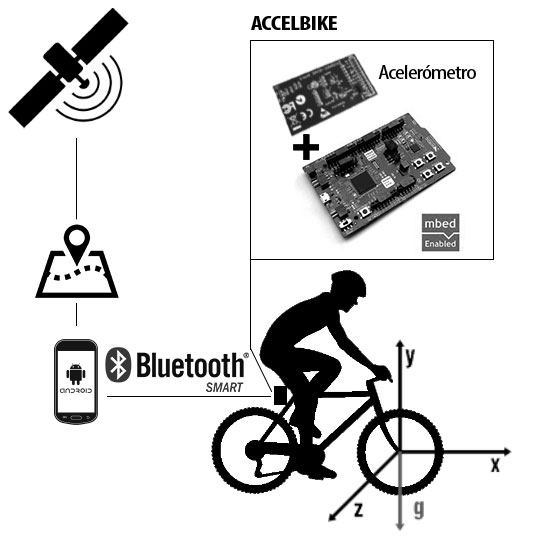
\includegraphics[scale=0.6]{figures/esquema_accelbike.jpg} % TODO hacer que esto no quede horrible
    \caption[Esquema del funcionamiento del proyecto]{Esquema del funcionamiento del proyecto. El dispositivo móvil recoge datos tanto de la localización como de un sensor de acelerometría.}
   	\label{figuraEsquemaAccelbike}
\end{figure}


%\begin{figure}[htb]%t=top, b=bottom, h=here
%
%    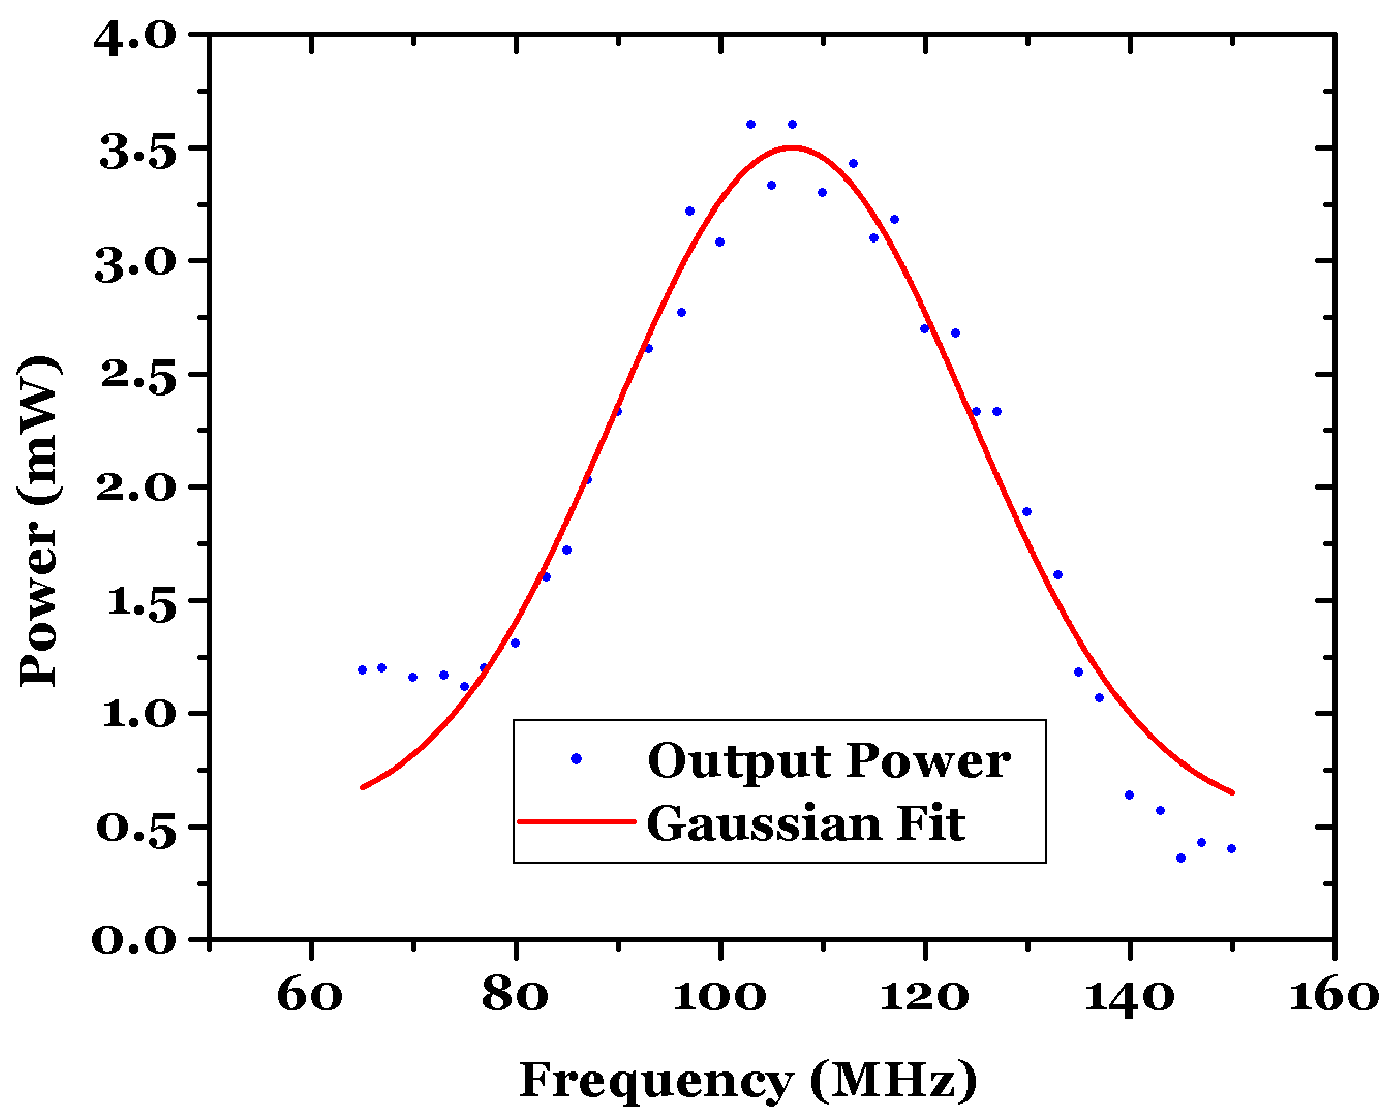
\includegraphics[height=2.5in]{figures/graph.png}
%
%    \caption[Optional: Short caption to appear in List of
%    Figures]{Full caption to appear below the Figure}
%
%   \label{figure1}
%\end{figure}

% +--------------------------------------------------------------------+
% |To create cross-references to figures, tables and segments
% |of text, LaTeX provides the following commands:
% |   \label{marker}
% |   \ref{marker}
% |   \pageref{marker}
% | where {marker} is a unique identifier.
% |
% | In the line above, we use \label{figure1} to mark a location
% | we wish to refer to later.  LATEX replaces \ref by the number of
% | the chapter, section, subsection, figure, or table after which the
% | corresponding \label command was issued. \pageref prints the page
% | number of the page where the \label command occurred.
% |
% +--------------------------------------------------------------------+

%Here is an example of a Table:

%\begin{table}

% +--------------------------------------------------------------------+
% | We include the command \begin{center} to center the table
% | horizontally on the page.  Note use of the command \end{center}
% | to turn off centering after the table is defined.
% +--------------------------------------------------------------------+
%    \begin{center}

% +--------------------------------------------------------------------+
% | The table is created with this command
% |
% | \begin{tabular}[pos]{table spec}
% |
% | The "pos" argument specifies the vertical position of the table relative to
% | the baseline of the surrounding text.  Use t, b, or c to specify alignment
% | at the top, bottom, or center.
% |
% | The "table spec" command defines the format of the table
% |   l for a column of left-aligned text
% |   r for a column of right-aligned text
% |   c for centered text
% |   p{width} for a column containing justified text with line breaks
% |   | for a vertical line
% +--------------------------------------------------------------------+

%    \begin{tabular}[c]{|c|c|c|}
%        \hline
%        Column 1 Heading & Column 2 Heading & Column 3 Heading \\
%        \hline
%        Col 1 Row 1 & Col 2 Row 1 & Col 3 Row 1\\
%        Col 1 Row 2 & Col 2 Row 2 & Col 3 Row 2\\
%        Col 1 Row 3 & Col 2 Row 3 & Col 3 Row 3\\
%        \hline
%    \end{tabular}
%    \caption{Caption to appear below the table}
%    \label{table1}
%   \end{center}
%\end{table}

% +--------------------------------------------------------------------+
% | Replace \section headings below with the title of your
% | subsections.  LaTeX will automatically number the subsections 1.1,
% | 1.2, 1.3, etc.
% +--------------------------------------------------------------------+

%In this paragraph, we want to refer to Fig.~\ref{figure1}
%mentioned at the beginning of this chapter.  We also refer to the
%Table~\ref{table1}.

%\section{Making a Reference to a Chapter Subsection}
%\label{makereference1.2}

%In this section, we refer back to text mentioned in
%Section~\ref{makereference1.1} on page~\pageref{makereference1.1}.

%\section{Making a Citation}
%\label{makereference1.3}

%Here's an example of a citation to a single
%work.~\citet{CT:Weiner:1999} It's also possible to make multiple
%citations.~\citet{CT:Phillips:1985, ARP:Loy:1974}


% +--------------------------------------------------------------------+
% | Uncomment the lines below to add additional chapters.  Name the
% | files chapter2.tex for Chapter 2, chapter3.tex for Chapter 3, etc.
% +--------------------------------------------------------------------+

% +--------------------------------------------------------------------+
% | Sample Chapter 2
% +--------------------------------------------------------------------+

\cleardoublepage

% +--------------------------------------------------------------------+
% | Replace "This is Chapter 2" below with the title of your chapter.
% | LaTeX will automatically number the chapters.
% +--------------------------------------------------------------------+

\chapter{Bluetooth Low Energy}
\label{makereference2}

Bluetooth Low Energy (BLE, también denominado Bluetooth Smart) empezó como parte de la Bluetooth 4.0 Core Specification. Diseñado originalmente por Nokia bajo el nombre de Wibree, fue luego adoptado por el Bluetooth Special Interest Group (SIG).~\cite{BLE:Townsend:2014}~\cite{BLE:Heydon:2012}~\cite{bluetoothCS}

El objetivo de Bluetooth Low Energy es complementar al Bluetooth clásico y ser la tecnología inalámbrica con el menor consumo energético posible. También tiene como objetivo llegar a una gran cantidad de objetos que hasta ahora no disponían de ninguna conectividad inalámbrica. Para lograr abarcar tantos escenarios, se necesita tener un coste muy bajo, lo cual se consigue con tres elementos clave:

\begin{itemize}

	\item \textbf{Banda ISM:} BLE utiliza la banda ISM (Industrial, Scientific and Medical) de 2,4GHz, que, a pesar de tener numerosos problemas como poco rango o interferencias por otras tecnologías como WiFi, etc, está disponible en todo el mundo con las mismas reglas y no tiene requisitos de licencia.

	\item \textbf{Licencia:} Cuando la tecnología Wibree estuvo lo suficiente madura como para unirse con un grupo de estándares inalámbricos, Nokia decidió elegir al Bluetooth Special Interest Group por su excelente reputación y su política de licencias. Esta política, comparada con la de otros grupos bajo la política Fair, Reasonable and Non-discriminatory, significa que los costes de licencia de un dispositivo Bluetooth se reducen significativamente. Con un menor coste de licencia se reduce el coste por dispositivo.

	\item \textbf{Bajo consumo:} La mejor forma de producir un dispositivo con bajo coste es reducir el coste de sus materiales, por ejemplo las baterías. Un dispositivo BLE puede funcionar perfectamente alimentado por una simple pila de botón CR2032.

\end{itemize}

\section{Comparación con Bluetooth Clásico}
\label{makereference2.1}

Aunque comparta con Bluetooth su nombre y mucha de la tecnología utilizada, se deben considerar diferentes tecnologías, ya que tienen objetivos de diseño completamente diferentes.

El Bluetooth clásico (también conocido como \textit{BR/EDR}~\cite{bluetoothCS}) se diseñó para conectar diferentes dispositivos, empezando por teléfonos móviles y ordenadores, y con el tiempo añadiendo más casos de uso como auriculares inalámbricos, streaming de música, impresión inalámbrica, etc. Cada uno de estos casos requería cada vez más ancho de banda, por lo que se fueron añadiendo radios cada vez más rápidas (la primera versión transmitía a 1 Mbps, aumentando a 3 Mbps en la versión 2.0, hasta los cientos de megabits por segundo en su versión 3.0)

Bluetooth Low Energy está optimizado para tener un consumo de energía muy bajo, por lo que se reduce el ancho de banda, y está pensado para aplicarse en dispositivos con un coste muy bajo, con una complejidad a su vez baja. Cada capa de su arquitectura se ha optimizado para reducir el consumo de energía al realizar una determinada tarea. Por ejemplo, relajando los parámetros de la radio usada por la capa física, comparándola con la radio del Bluetooth clásico, se puede usar menos energía cuando se está transmitiendo o recibiendo datos.

Precisamente por tener estos objetivos tan diferentes, Bluetooth clásico y BLE pueden coexistir en la misma aplicación en lo que se denomina \textit{Modo Dual} (en inglés \textit{Dual-Mode}), de modo que se puede conectar por ejemplo a unos auriculares inalámbricos por medio de BR/EDR mientras se accede a un dispositivo de bajo consumo, como un \textit{wearable}, por BLE.

\section{Tecnología}
\label{makereference2.2}

Un dispositivo BLE se divide en tres partes: controlador, anfitrión y aplicación. Cada una de estas partes se divide a su vez en distintas capas que proveen la funcionalidad necesaria para operar. En la Figura~\ref{figuraBLEHardware} se muestra un esquema de esta estructura.

\begin{figure}[h]%t=top, b=bottom, h=here
	\centering
    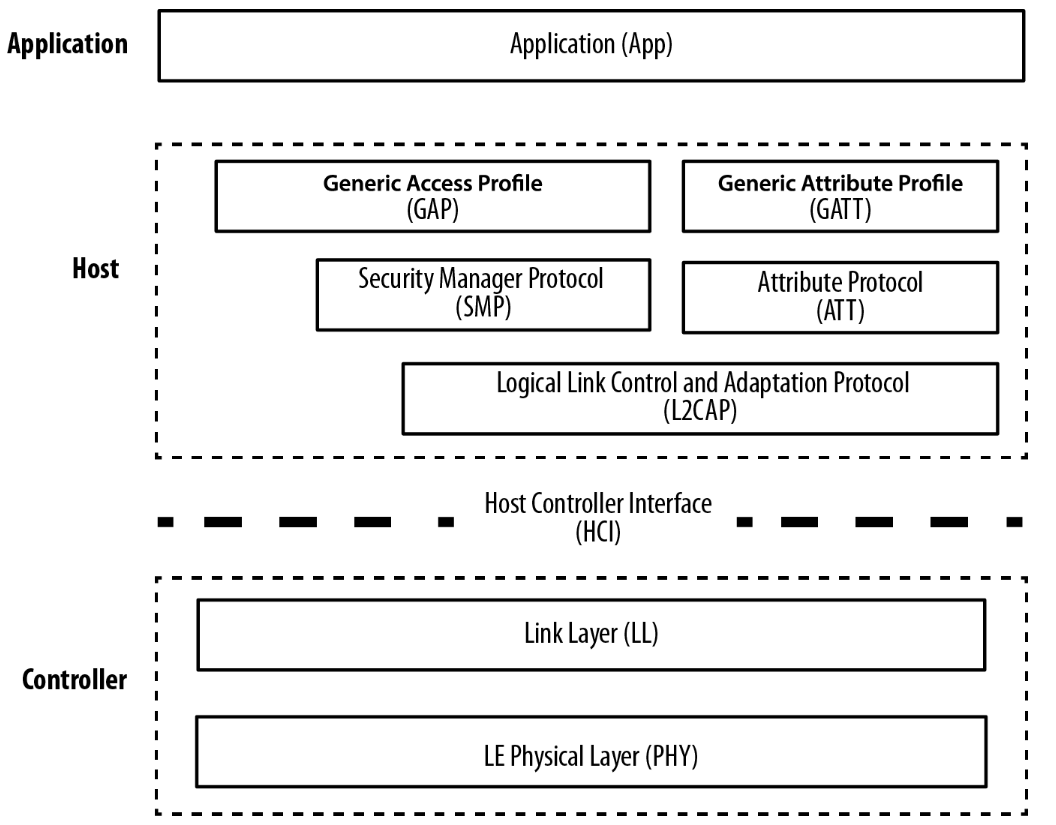
\includegraphics[scale=0.4]{figures/ble_hardware.png} % TODO hacer que esto no quede horrible
    \caption[Estructura hardware de un dispositivo BLE]{Estructura hardware de un dispositivo BLE}
   	\label{figuraBLEHardware}
\end{figure}

\subsection{Controlador}
\label{makereference2.2.1}

\textbf{Capa Física (Physical Layer, PHY).} La capa física es la que contiene los circuitos capaces de comunicarse de forma analógica, modulando y demodulando las señales analógicas y transformándolas en digitales.
Como ya se ha mencionado, la radio usada para BLE utiliza la banda ISM de 2,4 GHz. Esta banda se divide en 40 canales, desde los 2,4000 GHz hasta los 2,4835 GHz. De estos canales, 37 se utilizan para el envío de datos y los 3 restantes como canales de anuncio, para iniciar conexiones y mandar datos de broadcast.

\begin{figure}[h]%t=top, b=bottom, h=here
	\centering
    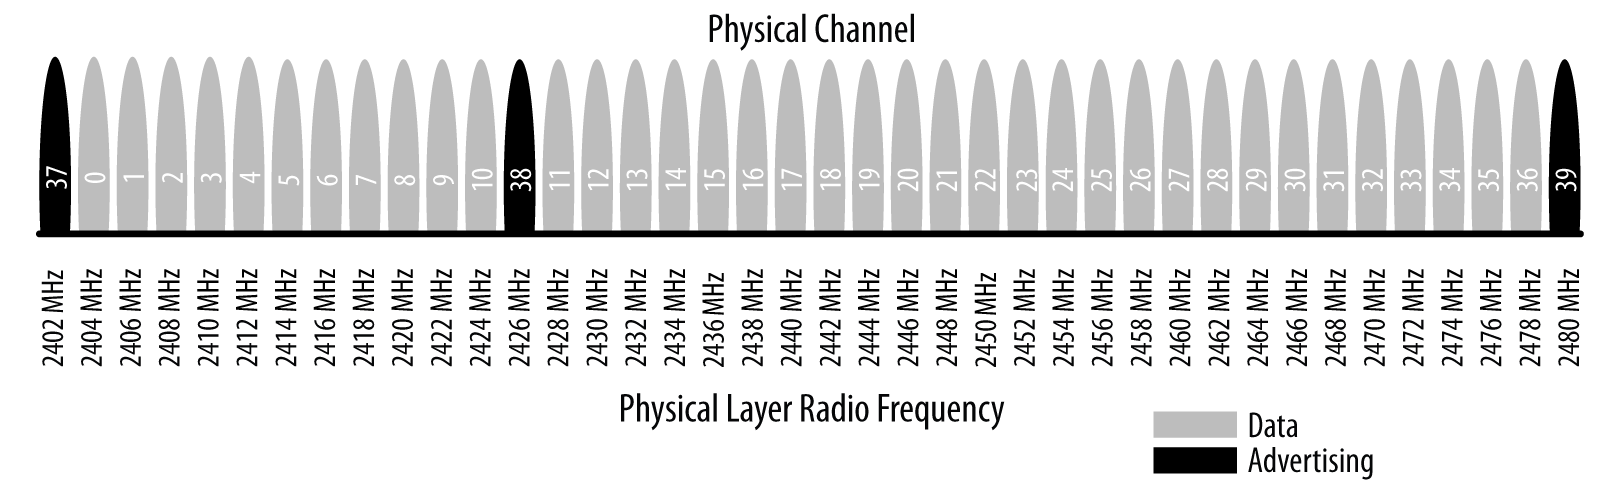
\includegraphics[width=\linewidth]{figures/ble_physical_layer.png} % TODO hacer que esto no quede horrible
    \caption[División de la banda de frecuencia ISM]{División de la banda de frecuencia ISM en 40 canales}
   	\label{figuraBLEPhysicalLayer}
\end{figure}

Para evitar interferencias con otros dispositivos transmitiendo en la misma banda, mayormente WiFi y Bluetooth clásico, el estándar BLE utiliza una técnica llamada \textit{frequency hopping spread spectrum}, que hace que la radio “salte” entre los distintos canales en cada conexión.


\textbf{Capa de Enlace (Link Layer).} Es la parte que actúa de interfaz de la capa física. Normalmente se implementa como una mezcla de software y hardware personalizado. Es responsable de anunciar, escanear, crear y mantener las conexiones. También se encarga de asegurar que los paquetes están correctamente estructurados. Por ello es probablemente la capa más compleja de la arquitectura BLE.


\textbf{Interfaz Anfitrión/Controlador (Host/Controller Interface, HCI).} Muchos dispositivos separan el Anfitrión del Controlador, y para estos casos, el HCI provee una interfaz estandarizada para comunicar los dos dependiendo del método de transporte físico de los datos. Entre estas interfaces se incluyen USB, SDIO o variantes de UART.

\subsection{Anfitrión}
\label{makereference2.2.2}

\textbf{Control Lógico de Enlace y Protocolo de Adaptación (Logical Link Control and Adaptation Protocol, L2CAP).} Esta capa provee dos funcionalidades: actúa como capa multiplexora de los protocolos, es decir, recibe los protocolos de las capas superiores y los encapsula en el formato de paquete estándar BLE (y viceversa). Asimismo, fragmenta los paquetes que se le envían desde las capas superiores para que quepan en los 27 bytes que tienen como máximo los paquetes de transmisión y vuelve a combinar los paquetes fragmentados que recibe.


\textbf{Protocolo de Atributos (Attribute Protocol, ATT).} Define una serie de reglas para acceder a los datos de un dispositivo. Propone una manera de encapsular estos datos en forma de \textit{atributos}, que permiten identificarlos asignando a cada uno un handle de 16 bits y un Identificador Único Universal (Universal Unique Identifier, UUID) y restringir su acceso mediante una serie de permisos. Los campos que forman un atributo se explicarán más adelante en la Sección~\ref{makereference2.4.2}. En resumen, ATT un protocolo muy simple, en el que un cliente puede acceder a los atributos de un servidor.\\
Para definir la comunicación eficaz de estos atributos entre el cliente y el servidor, ATT define seis tipos de mensajes:
\begin{itemize} % Hay imagenes de esto, por si no queda clarinete
	\item Solicitudes enviadas desde el cliente al servidor.
	\item Respuestas del servidor a una solicitud del cliente.
	\item Comandos enviados del cliente al servidor que no necesitan respuesta. 
	\item Notificaciones enviadas desde el servidor al cliente que no necesitan confirmación.
	\item Indicaciones enviadas desde el servidor al cliente.
	\item Confirmaciones enviadas por el cliente en respuesta a una indicación.
	\item De este modo ambos pueden establecer una comunicación con mensajes que requieran o no respuesta.
\end{itemize}


\textbf{Perfil de Atributo Genérico (Generic Attribute Profile, GATT).} Este perfil se asienta en el Protocolo de Atributos, y define los tipos de atributos y cómo se utilizan. 
Para ello utiliza una jerarquía de capas y un modelo de abstracción de datos. Los datos ahora se encapsulan en servicios, que a su vez consisten en una o más características que pueden estar definidas por un descriptor. Estas capas se sirven de metadatos para dar más información sobre los datos que se están manejando, como nombres, unidades, etc.\\
Este perfil es importante a la hora de comunicar dispositivos por BLE, y se usa como base para generar perfiles específicos para determinados casos de uso, como la medición del ritmo cardíaco de una persona o el acceso al nivel de batería disponible de un dispositivo. En la Sección~\ref{makereference2.4} se detallarán los componentes de un perfil GATT.


\textbf{Perfil de Acceso Genérico (Generic Access Profile, GAP).} Define cómo los dispositivos realizan procedimientos de control como el descubrimiento de otros dispositivos, conexiones entre éstos o la seguridad, es decir, dicta cómo interactúan dos dispositivos en un nivel más bajo.
GAP establece diferentes normas y conceptos para regular y estandarizar las operaciones a bajo nivel de los dispositivos:
\begin{itemize}
	\item Roles en los que los dispositivos pueden operar, estableciendo restricciones e imponiendo determinados comportamientos. Se explican con más detalle en las secciones~\ref{makereference2.3.1} y~\ref{makereference2.3.2}.
	\item Modos operacionales, que establecen estados a los que un dispositivo puede cambiar durante un determinado periodo de tiempo para lograr un objetivo, como por ejemplo permitir su descubrimiento o de qué modo permite realizar la conexión.
	\item Procedimientos operacionales para asegurar una comunicación constante mediante una secuencia de acciones.
	\item Aspectos de la seguridad, incluyendo modos y procedimientos.
	\item Formatos de datos adicionales para datos no protocolarios.
\end{itemize}


\textbf{Gestor de Seguridad (Security Manager, SM).} Define los protocolos y sus modos de operar para gestionar la integridad de los enlaces, la autenticación y el cifrado entre dispositivos Bluetooth, y provee las funciones de seguridad que se pueden utilizar para asegurar casi cualquier nivel de seguridad que sea necesario para las diversas aplicaciones.
 
\subsection{Aplicación}
\label{makereference2.2.3}

La aplicación es la capa más alta y la responsable de contener la lógica, la interfaz de usuario y el manejo de los datos de todo lo relacionado con el caso de uso particular que se esté implementando. Es por ello que su arquitectura dependerá en gran medida de la implementación particular. 

\section{Descubrimiento de dispositivos y enlazado}
\label{makereference2.3}

BLE tiene un único formato de paquete que soporta dos tipos: de datos y de anuncio; esto reduce la complejidad de la implementación de la pila de protocolos.

Los paquetes de anuncio tienen como propósito transmitir datos sin necesidad de una conexión o descubrir esclavos para iniciar una conexión. Tienen una capacidad útil de 31 bytes, que se utilizan para incluir información sobre el dispositivo y sus capacidades, pero también se pueden incluir los datos que se quieran transmitir. Estos paquetes se envían a intervalos definidos previamente, que pueden ir desde los 20 ms hasta los 10.24 s. Con un intervalo más corto se aumenta la frecuencia de envío de información, pero también significa que tiene un mayor consumo. En nuestro caso definimos un intervalo de 1 s.

Los paquetes de datos se utilizan una vez establecida una conexión para enviar información entre dos dispositivos. Tienen una capacidad de 27 bytes, menor que los de anuncio, debido a que los paquetes de datos ofrecen la posibilidad de encriptar el mensaje, para lo que se necesitan 4 bytes para la comprobación de la integridad del mismo. Para simplificar el diseño de la Capa de Enlace, los paquetes de datos que no utilicen encriptación también tienen ese \emph{overhead} de 4 bytes en la construcción del paquete.

Como explicamos anteriormente, BLE utiliza como máximo tres canales de frecuencia para mandar los paquetes de anuncio, y debido a que el dispositivo que anuncia y el que escanea no están sincronizados de ningún modo, los paquetes se recibirán cuando ambos se solapen aleatoriamente, como se ve en el ejemplo presentado en la Figura~\ref{figuraBLEScan}.

\begin{figure}[h]%t=top, b=bottom, h=here
	\centering
    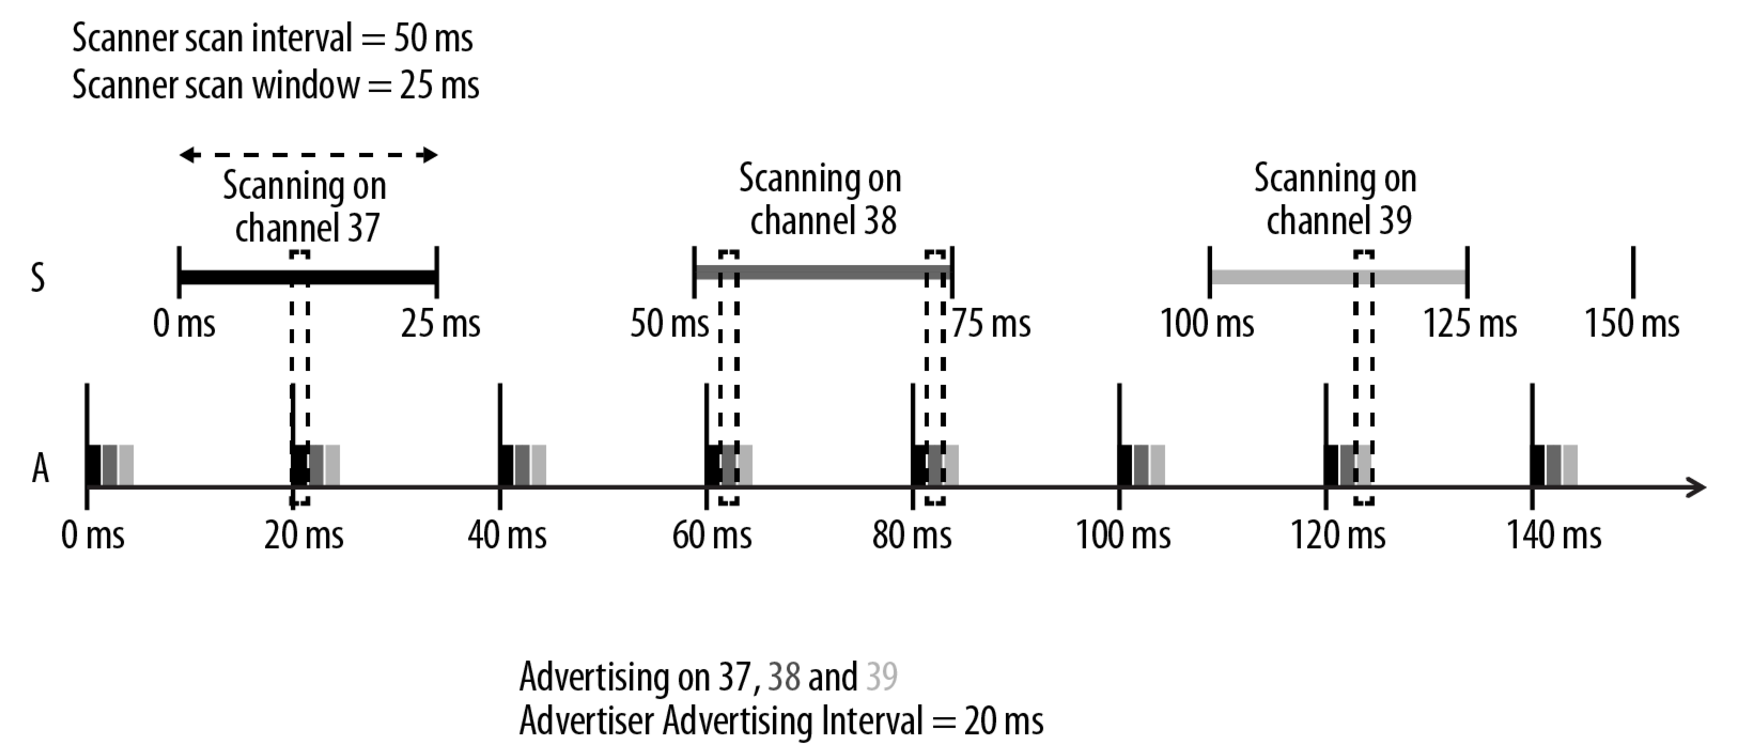
\includegraphics[width=\linewidth]{figures/ble_scan_example.png} % TODO hacer que esto no quede horrible
    \caption[Ejemplo de escaneo BLE]{Ejemplo de escaneo en BLE. El Scanner escanea cada 50 ms durante 25 ms en un canal determinado cada vez y el Advertiser anuncia cada 20 ms en los 3 canales. Cada vez que solapan se muestra con una línea de puntos.}
   	\label{figuraBLEScan}
\end{figure}

Un dispositivo BLE puede comunicarse con el mundo exterior mediante dos vías: \textbf{broadcasting} y \textbf{conexiones}.

\subsection{Modo Broadcast}
\label{makereference2.3.1}

Mediante broadcasting es posible enviar datos en un único sentido a cualquier dispositivo que esté escaneando en el radio de escucha. Es la única forma de mandar datos a más de un dispositivo a la vez, aunque no permite transmitir una gran cantidad de información.
 
Los dispositivos pueden tomar los siguientes roles GAP:
\begin{itemize}
	\item Broadcaster: envía periódicamente paquetes, sin importar si hay otros dispositivos escuchando.
	\item Observador: escanea las frecuencias establecidas para recibir estos paquetes. 
\end{itemize}

Como se ha explicado antes, el método utilizado para mandar información mediante broadcasting es el de los paquetes de anuncio. BLE permite enviar un segundo paquete por si se necesita mandar más información. Este método, llamado Scan Response, consiste en que el observador que encuentra la señal del broadcaster manda una petición para recibir el segundo paquete. Este segundo paquete de anuncio dispone de otros 31 bytes, haciendo un total de 62 bytes.

\begin{figure}[h]%t=top, b=bottom, h=here
	\centering
    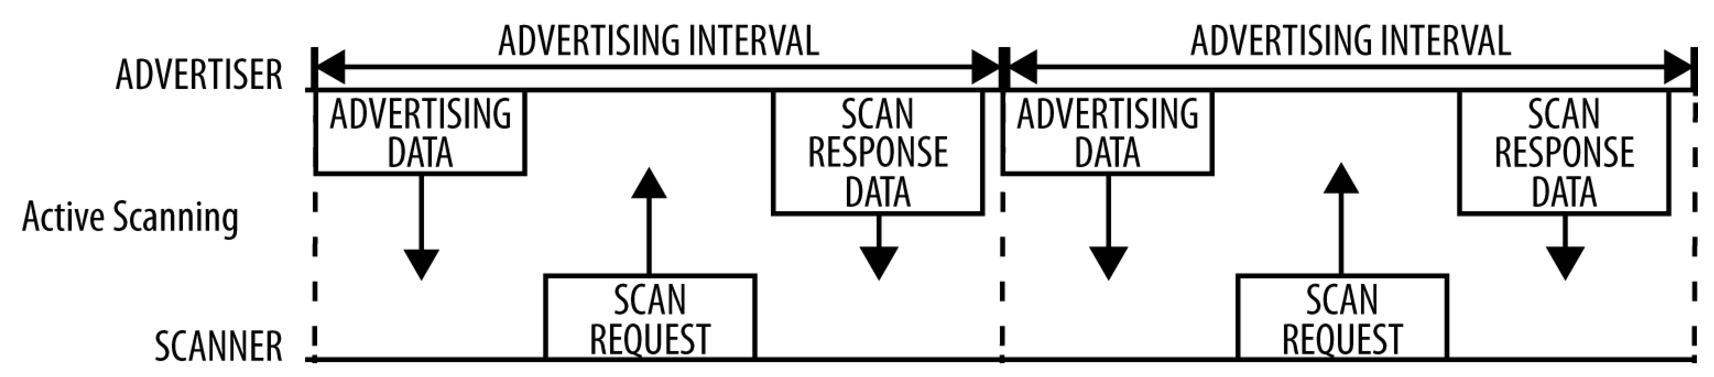
\includegraphics[width=\linewidth]{figures/ble_scan_response.png} % TODO hacer que esto no quede horrible
    \caption[Esquema de Scan Response]{Esquema de Scan Response. El dispositivo que escanea recibe un paquete de advertising y envía esta respuesta para requerir un segundo paquete con más información.}
   	\label{figuraBLEScanResponse}
\end{figure}

Si se desea que la comunicación se realice en los dos sentidos, o una mayor privacidad (dado que, en modo broadcast, todos los dispositivos que escuchan reciben la misma información), o bien se necesita enviar más datos de los que es posible con el modo broadcast, tendremos que usar el modo conexión.

\subsection{Modo Conexión}
\label{makereference2.3.2}

Una conexión permite un intercambio de paquetes de forma periódica y permanente entre dos dispositivos. En este modo tenemos dos roles GAP:

\begin{itemize}
	\item Central (maestro): escanea las frecuencias predefinidas en busca paquetes de advertising y es el encargado de realizar las conexiones. Una vez conectado, es el encargado de gestionar la sincronización y de iniciar el envío periódico de datos. Dado que los requisitos computacionales del rol de maestro son mayores que los de los esclavos, este rol suele recaer en los dispositivos con una CPU y memoria más avanzados, como un smartphone o una tablet.

	\item Periférico (esclavo): se encarga de enviar los paquetes de advertising para que los centrales puedan encontrarlos y de aceptar las conexiones entrantes. El protocolo BLE está optimizado para requerir pocos recursos, en términos de energía y memoria, para la implementación de este rol.
\end{itemize}

La principal ventaja de las conexiones es la posibilidad de organizar los datos que se envían mediante el uso de protocolos para cada campo, más específicamente el Generic Attibute Profile (GATT), que organiza los datos dentro de servicios y características.

\section{Generic Attribute Profile (GATT)}
\label{makereference2.4}

El Perfil de Atributo Genérico expande el Protocolo de Atributo (ATT) estableciendo en detalle cómo intercambiar todos los datos del usuario a través de una conexión BLE. También provee un \textit{framework} para todos los perfiles basados en GATT, que cubren casos de uso específicos y asegura el intercambio entre dispositivos de diferentes marcas. Todos los perfiles BLE estándar están basados en GATT y deben cumplir sus especificaciones para operar correctamente.

\subsection{Roles}
\label{makereference2.4.1}

GATT define dos roles que pueden adoptar los dispositivos interconectados, que hereda directamente del Protocolo de Atributos (ATT):
\begin{itemize}
	\item \textbf{Cliente.} Envía peticiones al servidor y recibe respuestas. El cliente GATT no tiene conocimiento sobre los atributos del servidor por adelantado, por lo que primero tiene que recopilar información sobre éstos mediante un descubrimiento de servicios.

	\item \textbf{Servidor.} Recibe las peticiones del cliente y responde en consecuencia. Es el rol responsable de guardar los datos y de hacer que estén disponibles para el cliente, organizándolos en atributos. Todos los dispositivos BLE que se vendan deben incluir al menos un servidor GATT básico, aunque únicamente envíe un error como respuesta.
\end{itemize}

\subsection{Jerarquía de datos}
\label{makereference2.4.2}

ATT define el protocolo de atributos, cómo se estructuran y se pueden usar para intercambiar información sobre dispositivos, pero no ofrece más estructura. GATT va más allá y establece una jerarquía de datos estricta para organizar los atributos y permitir su reutilización, de modo que el acceso de información entre cliente y servidor siga una serie de reglas que se puedan usar en cualquier perfil basado en GATT.

\begin{figure}[h]%t=top, b=bottom, h=here
	\centering
    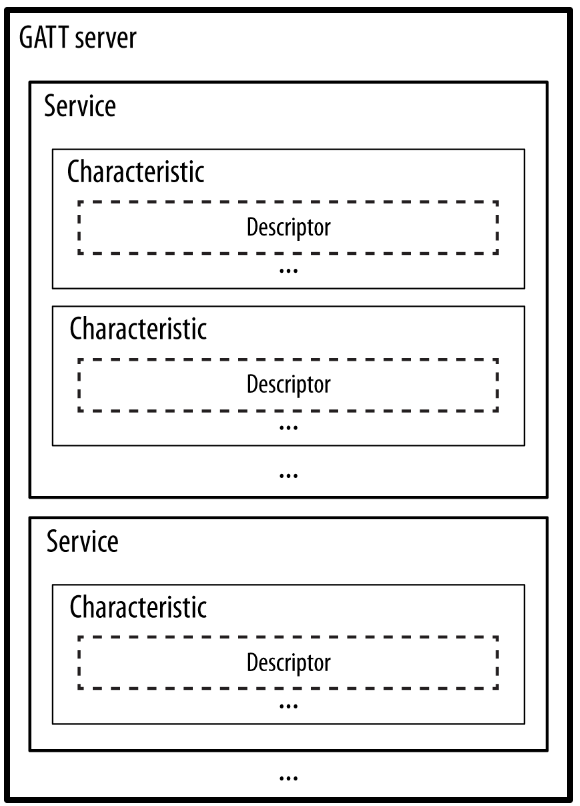
\includegraphics[scale=0.5]{figures/ble_gatt_hierarchy.png} % TODO hacer que esto no quede horrible
    \caption[Esquema de la estructura de datos de GATT]{Esquema de la estructura de datos de GATT}
   	\label{figuraBLEGATTHierarchy}
\end{figure}

Un perfil basado en GATT tendrá entonces, como se muestra en la Figura~\ref{figuraBLEGATTHierarchy}, como mínimo un servicio, con una o más características que encapsulan a los atributos, y que pueden añadir más información a través de un descriptor.\\
De esta forma, si tenemos por ejemplo un dispositivo del que nos interesa sacar información sobre un sensor de temperatura y obtener el estado de la batería, tendríamos la siguiente estructura:
\begin{itemize}
	\item Un \textbf{servicio} para la temperatura y otro para el nivel de batería.
	\item Dentro de cada servicio, una \textbf{característica} que encapsule ambos valores.
	\item De manera opcional, se puede agregar un \textbf{descriptor} dentro de alguna de las características.
\end{itemize}
Cada uno de estos niveles ofrece un modo de identificarlos y más información sobre ellos, por lo que un cliente que no conozca de qué servicios dispone un servidor, puede realizar lo que se denomina una \textit{exploración de servicios} y así conocer qué información puede obtener. Todos los niveles se especifícan mediante atributos, ya que es la base sobre la que se asienta GATT, por ello es necesario definir primero en qué consiste un atributo.\\

\textbf{Atributo.} Los atributos son las entidades de datos más pequeñas definidas en GATT y ATT. Son piezas de información direccionables que pueden contener los datos del usuario o metadatos sobre la estructura y el agrupamiento de cada una de las capas.

Dado que GATT y ATT sólo pueden operar con atributos, los clientes y servidores que deseen realizar una interacción deberán organizarse de esta forma. Cada atributo contiene los datos del usuario e información sobre el propio atributo, contenidos en los siguientes campos:
\begin{itemize}
	\item \textit{Handle.} Es la parte que hace a un atributo direccionable. Consiste en un identificador de 16 bits para cada atributo en un servicio GATT particular, y se garantiza que no se modificará entre transacciones o conexiones.  El valor 0x0000 denota un handle inválido, por lo que el rango de handles disponible es de 0xFFFF (65535), aunque en la práctica el número de atributos en un servidor es más cercano a la docena.

	\item \textit{Tipo.} Esta parte consiste en un UUID de 16, 32 o 128 bits que determina qué tipo de datos están presentes en el campo de valor del atributo, permitiendo por ejemplo mecanismos para encontrar un atributo directamente por su tipo. En la Sección~\ref{makereference2.4.3} se muestra cómo se forman los UUIDs para su uso en BLE.

	\item \textit{Permisos.} Los permisos son metadatos que especifican qué operaciones se pueden ejecutar en cada atributo y con qué requisitos de seguridad. ATT y GATT definen los siguientes permisos:
	\begin{itemize}
		\item Permisos de acceso: similares a los permisos presentes en un archivo.  Define si se puede acceder a un valor como sólo de lectura, de escritura, de ambos o de ninguno.
		\item Encriptación: determina si es necesario algún nivel de encriptación para acceder al valor. Puede no necesitarla, o exigir una encriptación con o sin autenticación.
		\item Autorización: determina si se necesita o no permiso del usuario para acceder al atributo.
	\end{itemize}

	\item \textit{Valor.} Contiene los propios datos sin restricción de qué tipo sean, aunque con un máximo de 512 bytes según la especificación. Dependiendo del tipo de atributo, puede contener información adicional sobre el atributo o un valor útil.
\end{itemize}

\textbf{Servicio.} Los servicios agrupan atributos conceptualmente relacionados. La forma de definir un servicio es a través de uno o más atributos denominados \textit{definición de servicio}, de los cuales el primero es el que actúa de declaración de servicio y el resto pueden definir las siguientes capas, como características y descriptores.

Se puede comparar un servicio con una clase en cualquier lenguaje de programación orientado a objetos. 

\textbf{Característica.} Las características se pueden entender como contenedores para los datos del usuario. Siempre incluyen dos atributos: la \textit{declaración de la característica}, que ofrece metadatos sobre los datos en sí, y el \textit{valor de la característica}, que es un atributo completo con los datos del usuario. Adicionalmente, una característica puede contener un descriptor, que es un atributo que provee de más metadatos.

\textbf{Descriptor.} Se utilizan principalmente para proveer al cliente con información adicional sobre las características y su valor. Se ubican siempre entre la definición de la característica y el valor del atributo de la característica y están compuestos por un único atributo cuyo UUID define el tipo de descriptor y el campo de valor contiene lo que esté definido para ese tipo de descriptor.

A continuación se detallan algunos de los descriptores más utilizados:

\begin{itemize}
	\item \textit{Descriptor de usuario de una característica:} contiene una descripción que el usuario puede leer consistente en una cadena de caracteres en UTF-8. Por ejemplo “Temperatura en el salón”.
	\item \textit{Descriptor de configuración de la característica por el cliente:} actúa como un “interruptor”, deshabilitando las actualizaciones que envía el servidor.
	\item \textit{Descriptor de formato de presentación de una característica:} contiene el tipo de variable de la característica, por ejemplo booleano, cadena de caracteres, enteros, etc.
\end{itemize}

\subsection{UUIDs}
\label{makereference2.4.3}

Un \textit{Identificador Único Universal} (UUID) es un número de 128 bits (16 bytes) que garantiza (al menos con una gran probabilidad) que es único globalmente. UUID es usado en otros protocolos aparte de Bluetooth, y su formato, uso y generación se especifican en el ISO/IEC 9834-8:2005.

Dado que 16 bytes ocuparía gran parte del tamaño disponible en los 27 bytes de los paquetes de datos, la especificación BLE añade dos formatos adicionales: UUIDs de 16 o 32 bits, y se forman definiendo un “final” del UUID que es constante en todos los dispositivos BLE, en los que se sustituyen los 32 primeros bits:

\begin{center}xxxxxxxx-0000-1000-8000-00805F9B34FB\end{center}

donde xxxxxxxx son los bits a sustituir.


%In this chapter, I want to refer to Chapter~\ref{makereference},
%so I'm going to use the slash ref command along with the
%"makereference" label which I assigned back at the beginning of
%Chapter 1.

%\section{Page Number References}
%\label{makereference2.1} I should also be able to refer to a
%specific page number, such as page~\pageref{makereference}.  Of
%course, I'll need to have a slash label command and a unique name
%in each section that I want to be able to refer to later in the
%text.

%\section{Referring to Sections Within Chapter 1}
%\label{makereference2.2} Now, I'm going to refer to different
%sections within Chapter 1. I gave an example of a figure in
%section~\ref{makereference1.1} and an example of a table in
%section~\ref{makereference1.2}.  In
%section~\ref{makereference1.3}, we looked at examples of
%bibliographic citations.

% +--------------------------------------------------------------------+
% | Sample Chapter 3
% +--------------------------------------------------------------------+

\cleardoublepage

% +--------------------------------------------------------------------+
% | Replace "This is Chapter 3" below with the title of your chapter.
% | LaTeX will automatically number the chapters.
% +--------------------------------------------------------------------+

\chapter{Exploración Hardware}
\label{makereference3}

El primer hito a nivel técnico era encontrar una placa de desarrollo que incluyera Bluetooth de bajo consumo y permitiera conectar un sensor de acelerometría, ya que eran indispensables para la transmisión de datos entre la placa y el dispositivo móvil. 

Desde el punto de vista comercial, la intención ha sido buscar el componente con mejores prestaciones en calidad y precio con el objetivo de preparar un producto final que pudiera competir con otras opciones del mercado.

Destacamos las placas con Bluetooth incorporado y un microprocesador. En las tabla~\ref{tablaSoCBLE} observamos el análisis de cada elemento que se ha considerado.

\begin{table} % TODO marcar en un color las opciones elegidas
	\begin{center}
	\begin{tiny}
	\begin{tabular}[c]{|c|c|c|c|c|c|}
        \hline
        \multicolumn{6}{|c|}{CHIPS CON BLUETOOTH} \\
        \hline
        EMPRESA & MODELO & PROCESADOR & FLASH & RAM & I/O \\
        \hline
        Nordic & PTR9022 & ARM Cortex-M0 & 256 KB & 16 KB & SPI, 2-WIRE, UART \\
		Nordic & nRF51822 & ARM Cortex-M0 & 256/128KB & 32KB/16KB & SPI Master/Slave, 2-wire, UART, 31 GPIO \\
		Nordic & nRF51422 & ARM Cortex-M0 & 256/128KB & 16KB & SPI Master/Slave, 2-wire, UART, 31 GPIO \\
		TI & CC2540 / CC2541 & 8051 & 128/256KB & 8KB & 2 USART, ADC, 21 GPIO, SPI \\
		TI & CC2640F128RGZT & ARM Cortex-M3 & 128KB & 20KB & I2C, I2S, SPI, UART \\
		Cypress & 4 BLE/PRoC BLE & ARM Cortex-M0 & 128/256KB & 16/32KB & 2 SCBs, configurable como I2C, SPI o UART \\
		Cypress & PSoC 4XX7-BLE & ARM Cortex-M0 & 128KB & 16KB & I2C, SPI, UART, 36 GPIO \\
    	\hline
	\end{tabular}
	\end{tiny}
    \caption{Placas que integran radio Bluetooth Low Energy. Se destacan las alternativas seleccionadas para la siguiente fase de exploración}
    \label{tablaSoCBLE}
   \end{center}
\end{table}

Dada la naturaleza de nuestro proyecto no necesitábamos un gran poder de procesamiento ni una gran capacidad en cuanto a memoria RAM y flash, ya que el código iba a ser muy sencillo. Los dos factores principales a tener en cuenta eran que incorporase la tecnología Bluetooth Low Energy y que permitiese la conexión y el envío de datos con el acelerómetro, ya fuera mediante I2C, SPI, UART...

Realizando el primer filtro pudimos observar que algunas características eran comunes entre los SoC’s elegidos:

En materia de procesadores encontramos dos opciones comunes: \textbf{Cortex-M0} de ARM (Advanced RISC Machines) y \textbf{8051} de Intel. Al ver que la mayoría de los chip elegidos montaban el procesador de ARM, claramente observamos que domina el mercado de los sistemas empotrados y las empresas han optado por utilizarlo. Esto se debe a que el modelo de negocio utilizado por ARM consiste en la venta de licencias de sus núcleos~\cite{ARMIPCore}, lo que permite a otros fabricantes diseñar su propio System On Chip (SoC) integrando tecnología ARM.

ARM Cortex-M0 nos parecía una opción más interesante, ya que este procesador cuenta con la tecnología RISC, acrónimo de Reduced Instruction Set Computing, computación de instrucciones reducidas, cuenta con una arquitectura de 32 bits frente a los 16 de Intel 8051 y soporta la arquitectura Thumb, que mejora la densidad del código para ocupar menos espacio tanto en memoria RAM como en flash.

La cantidad de memoria RAM disponible más común para este tipo de dispositivos es de 8, 16 o 32 kilobytes. La segunda opción nos pareció más que suficiente para albergar un programa sencillo como el nuestro y las variables necesarias.

En cuanto a capacidad de almacenamiento, todas las placas cuentan con memoria flash, que pueden variar entre 128 y 256 Kilobytes. De nuevo, la complejidad de nuestro programa no iba a generar un fichero compilado de gran tamaño, y no necesitábamos guardar nada más, por lo que 128 KB nos parecieron adecuados.

En cuanto a los periféricos de entrada/salida, la mayoría de las placas de desarrollo incluyen los protocolos SPI e I2C.

El protocolo SPI consiste en el envío de la señal de reloj del maestro y en cada impulso de reloj se envía un bit al esclavo y recibe un bit de éste. Los nombres de las señales son SCK para el reloj, MOSI para el Maestro Out Esclavo In, y MISO para Maestro In Esclavo Out.

El protocolo I2C, usa dos cables, uno para el reloj (SCL) y otro para el dato (SDA). El maestro y esclavo envían datos por el mismo cable, el cual es controlado por el maestro, que crea la señal de reloj. Este protocolo utiliza direccionamiento, es decir, el primer byte enviado por el maestro se forma de 7 bits para la dirección (así que permite comunicarse con hasta 127 dispositivos) y un bit de lectura/escritura, indicando si el próximo byte vendrá desde el maestro o el esclavo. Esta tecnología se ampliará en el Capítulo~\ref{makereference4.8}.

\section{Análisis de los candidatos}
\label{makereference3.3}

Una vez recopilados los modelos de que observamos en la Tabla~\ref{tablaSoCBLE}, hemos destacado 2 placas de prototipado que cumplen con los requisitos del proyecto. Este tipo de placas ofrecen más características de las que necesitamos para el proyecto, pero suponen un primer paso para poder programar y realizar pruebas antes de pasar a chips más simples y con un menor coste. 

Por un lado escogimos la placa de desarrollo de Cypress con el kit PSoC BLE y modelo de la placa con Bluetooth \textbf{CY8CKIT-042-BLE} certificado para sistemas de bajo consumo. Es un kit provisto de un chip que ofrece un procesador ARM Cortex-M0 y capacidad y conectividad suficiente como para utilizarlo de base para el proyecto.

El entorno de desarrollo para las plataformas de Cypress es un software de escritorio llamado \textit{PSoC Creator}, en el cual podemos diseñar sistemas a través de un panel gráfico. Nos ofrece multitud de librerías disponibles para la placa utilizada y es posible codificar, compilar, y depurar código.\\

Consideramos también la placa de Nordic modelo \textbf{nRF51-DK} por ser un kit de desarrollo que ofrece el mismo procesador que Cypress, conectividad tanto I2C como SPI para realizar las pruebas con el sensor. 
Este modelo ofrece compatibilidad con la plataforma de desarrollo \textit{mbed} de ARM, es una opción que nos resultó interesante a la hora escogerla. Dispone de una gran comunidad y soporte lo cual es de agradecer.\\

En la Sección~\ref{makereference3.4} hablaremos más sobre los aspectos específicos de ambos entornos de desarrollo.

Al considerar que era más interesante tener una placa con procesador, sensores y periféricos descartamos los chips individuales y optamos por una opción más completa.

\section{Plataformas escogidas}
\label{makereference3.4}

Rápidamente observamos dos grandes empresas especializadas en el sector como son Nordic y Cypress. Tienen gran variedad de microprocesadores y placas de desarrollo que cumplen con nuestras expectativas.

Elegimos el kit de desarrollo de Nordic (\textbf{nRF51-DK}), que incluye Bluetooth Smart e incorpora un núcleo ARM Cortex-M0 32-bit como la mayoría de los chips que encontramos. Una memoria flash a 256/128KB con RAM de 32KB/16KB para mejorar el rendimiento de las aplicaciones.

El kit permite el acceso a todas las interfaces de entrada y salida como SPI Master/Slave, 2-wire, UART y 31 GPIOs a través de conectores. Tiene 4 LED’s y ofrece también 4 botones que son programables por el usuario. 

Utiliza un cable micro USB 2.0 para conectarse a uno de los puertos USB de el PC. Esto proporciona alimentación a la placa, y es compatible con la programación de destino.

\begin{figure}[h]%t=top, b=bottom, h=here
	\centering
    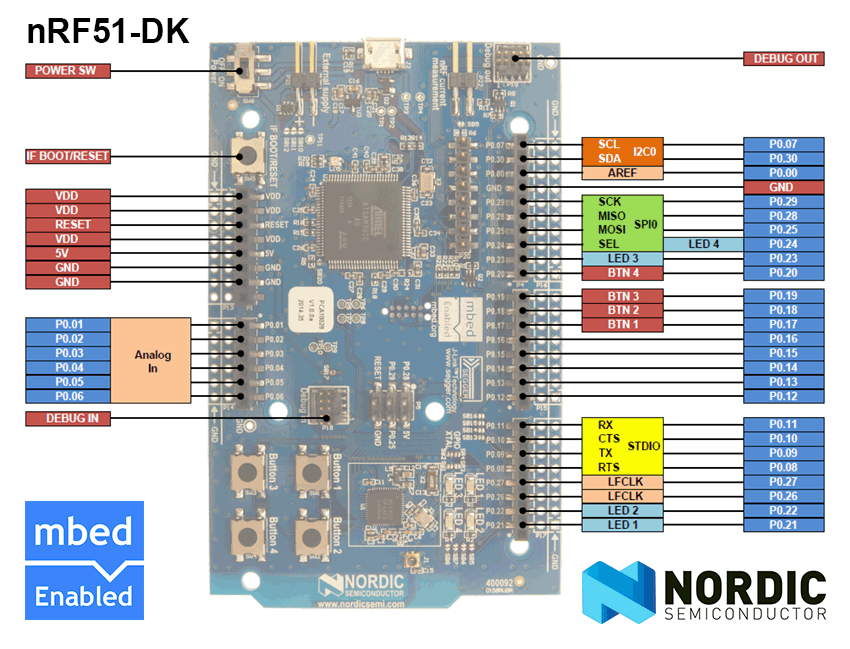
\includegraphics[scale=0.5]{figures/nRF51DK_pines.png} % TODO hacer que esto no quede horrible

    \caption[Esquema de la disposición de pines de la placa nRF51-DK de Nordic]{Esquema de la disposición de pines de la placa nRF51-DK de Nordic}

   \label{figuraNordicNRF51}
\end{figure}

La  carga de programas resulta sencilla, ya que solo debemos abrir un explorador de archivos de Windows. Confirmar que el nRF52 DK ha aparecido como una unidad extraíble llamado "JLINK". Esto permite programar el chip a bordo. Podremos cargar los programas a la placa arrastrando y soltando hacia la unidad.

\textbf{ARM Mbed} es una plataforma gratuita de prototipado rápido y experimentación con microcontroladores ARM. Provee a los desarrolladores una plataforma productiva para realizar pruebas conceptuales y prototipos en lenguaje de programación C/C++. Incluye amplia variedad de librerías, tutoriales y ejemplos, además de contar de una gran comunidad online de más de 130.000 desarrolladores de software, cuyos códigos son habitualmente accesibles a toda la comunidad.

Otro chip con procesador que nos pareció interesante fue el modelo CY8CKIT-042-BLE de la empresa Cypress que soporta 2 dispositivos: PSoC 4 BLE y  PRoC BLE.

El modelo escogido es el PSoC 4 BLE que provee de una completa solución para conectividad Bluetooth Low Energy. También monta una procesador ARM Cortex-M0 con una memoria flash de 128kB / 256kB y RAM de 16kB / 32kB. Dispone de 4 TCPWM1, 2 SCBs2, LCD4, I2S5, and 36 GPIOs.

\begin{figure}[h]%t=top, b=bottom, h=here
	\centering
    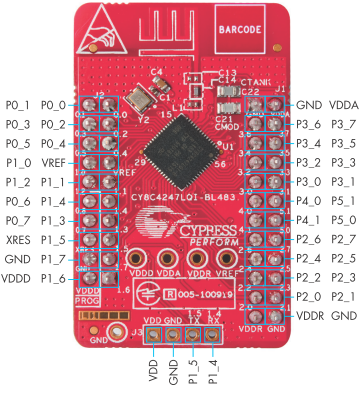
\includegraphics[scale=0.6]{figures/cypress_psoc.PNG} % TODO hacer que esto no quede horrible

    \caption[Cypress PSoC]{Cypress PSoC. Esta placa contiene el microchip y todos los conectores necesarios como para usarla directamente como producto final}

   \label{figuraCypressPeque}
\end{figure}

\begin{figure}[h]%t=top, b=bottom, h=here
	\centering
    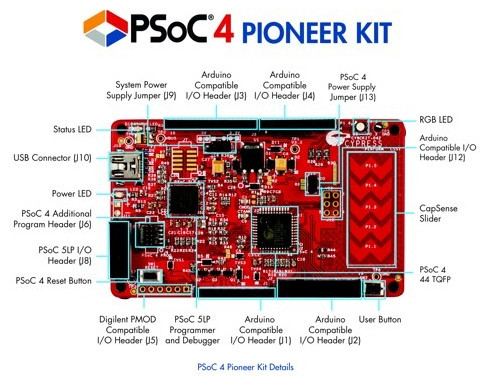
\includegraphics[width=\linewidth]{figures/cypress_placa_desarrollo} % TODO hacer que esto no quede horrible

    \caption[PSoC 4 BLE, placa de desarrollo]{PSoC 4 BLE, placa de desarrollo, en esta placa se conecta el PSoC para poder programarlo, y añade más funcionalidad incorporando elementos como botones programables, un LED RGB, un panel deslizante, etc.}

   \label{figuraCypressGrande}
\end{figure}

El kit incluye una memoria extraible que conecta la placa por Bluetooth llamado Dongle USB CySmart (BLE Dongle) que se empareja con la herramienta de emulación principal CySmart. El emparejamiento con un entorno Windows hace que sea un potente entorno de depuración de Bluetooth LE.

Este kit de desarrollo de Cypress es compatible con diseños a nivel de sistema mediante PSoC Creator, un software de desarrollo que contiene numerosos proyectos de ejemplo para proporcionar diseños integrados de señal mixta Bluetooth de baja energía, el lenguaje utilizado es C.

Es sencilla diseñar pues con arrastrar y soltar los componentes se añaden al panel principal obteniendo máxima flexibilidad de diseño.

\section{Conclusión}
\label{makereference3.5}

Tanto la placa nRF51-DK de Nordic como CY8CKIT-042-BLE de Cypress son dos placas de desarrollo perfectas para iniciar un proyecto con conectividad Bluetooth, las dos tienen idénticas características, conectores y periféricos, se les puede incluir una pila de botón CR2032 para darles autonomía y les respalda un software para desarrollo de las mismas.

En este punto tuvimos cierta controversia, ya que el software de Mbed de Nordic nos da la posibilidad de compilar código C++ en cualquier PC con internet gracias a su versión web. Nos ofrece una gran comunidad que es de agradecer y mucho contenido de ejemplos y tutoriales en la web oficial. Por contra no tiene modo depuración por pasos y eso dificulta su seguimiento y depuración. 

Por otro lado, PSoC Creator de Cypress nos ofrece un completo programa de escritorio muy visual al diseñar circuitos y un sistema “drag and drop” muy intuitivo. Permite modo depuración facilitando su programación. Por contra nos hemos encontrado con ciertas dudas que han sido difíciles de resolver en foros debido al poco contenido sobre el tema.

Debido al gran parecido entre las características de una placa y otra, y a que los entornos de desarrollo tienen cada uno sus pros y sus contras, nos resultó difícil elegir una de las dos para finalizar el proyecto. En el Capítulo~\ref{makereference4} se hablará de las pruebas que realizamos con ambas y qué nos motivó a escoger la placa de Nordic frente a la de Cypress.

\cleardoublepage

\chapter{Desarrollo Hardware}
\label{makereference4}

Antes de comenzar programando la funcionalidad principal de este proyecto tuvimos que aprender a utilizar herramientas y conceptos, como los entornos de desarrollo de las placas de Nordic y de Cypress o los protocolos SPI e I2C y el propio BLE, con los que no habíamos trabajado nunca, por lo que primero realizamos una serie de pruebas para familiarizarnos y así decidir cuál de ellas elegiríamos finalmente para el proyecto.

\section{Pruebas iniciales con Cypress y Nordic}
\label{makereference4.1}

Una vez tuvimos las placas, el primer paso fue buscar códigos de ejemplo con funcionalidades parecidas a lo que íbamos a tratar en el proyecto.

\textbf{Cypress} pone a disposición de cualquier desarrollador que desee realizar pruebas un repositorio en GitHub con 100 proyectos que sirven de ejemplo para utilizar la funcionalidad BLE de sus dispositivos PSoC. Aparte han desarrollado una aplicación Android llamada \textit{CySmart} para comprobar el funcionamiento de algunos de estos ejemplos.

\textbf{mbed} dispone de un repositorio propio donde cualquier usuario puede subir proyectos para cualquier dispositivo compatible con mbed. Estos proyectos son muy sencillos de buscar e importar desde el propio compilador. ARM mbed también dispone de una app Android, ésta llamada \textit{nRF Master Control Panel}, que permite hacer algunas pruebas.

Como primera toma de contacto con las posibilidades de las placas para comunicarse físicamente con otros dispositivos realizamos un pequeño circuito consistente en una fotoresistencia conectada a un conversor analógico-digital MCP3008, capaz de convertir una entrada analógica de voltaje en un valor binario, el cual se transmitiría por el bus SPI.

Una vez creado el circuito comprobamos con un voltímetro que dejar pasar menos luz sobre la fotoresistencia disminuía la cantidad de voltaje. El rango de voltaje que pudimos comprobar fue de 0,82 V a 1,82 V con luz ambiente.

\begin{figure}[h]%t=top, b=bottom, h=here
	\centering
    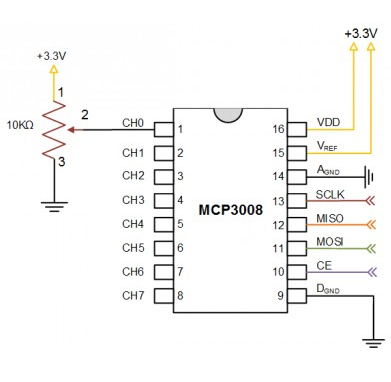
\includegraphics{figures/mcp3008_esquema.PNG} % TODO hacer que esto no quede horrible
    \caption[TODO]{TODO}
   	\label{figuraMCPEsquema}
\end{figure}

Para realizar la transferencia de datos por SPI colocamos como master la placa de desarrollo y como esclavo el circuito de la fotoresistencia. Conectamos los 4 pines correspondiente en cada de placa: para la trasmisión de datos (MOSI, MISO), frecuencia de reloj (SCLK) y selección del esclavo (nSS). Ambos entornos de desarrollo ofrecen ejemplos de módulo SPI con lo que fue fácil hacer funcionar el sistema una vez conectados los pines correctos.

Para comprobar en un principio si se recibían bien los datos, en la placa nRF51-DK de Nordic utilizamos sus 4 LED’S verdes, apagándolos o encenciéndolos según el valor ya digitalizado que recibe. De igual forma al probarlo con PSoc BLE de Cypress interactuamos con su LED RGB, utilizando los colores verde, azul y rojo para representar los diferentes datos que recibía del circuito.

Estas primeras pruebas nos sirvieron para comprobar la correcta recepción de datos, pero el objetivo era llevarlos a una aplicación desarrollada en Android. Por tanto nuestra primera toma de contacto con el desarrollo de la aplicación Android (Figura~\ref{figuraAPPPrueba}) que hacía uso del módulo BLE fue en este momento, centrado más en la funcionalidad más que en el diseño. Esta aplicación funcional nos permitió probar conceptos como el de activar desde dentro de una app el Bluetooth del móvil, realizar un escaneo para detectar los dispositivos con Bluetooth cercanos, conectarse a éstos y enviar datos. Para verificar que funcionaba correctamente, escribimos mensajes de log  que se pueden visualizar en el entorno de desarrollo Android Studio.

\begin{figure}[h]%t=top, b=bottom, h=here
	\centering 	
    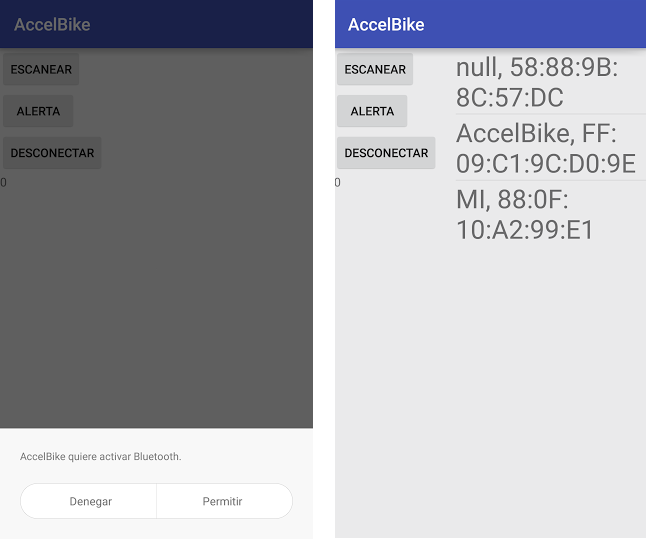
\includegraphics[width=\textwidth]{figures/app_piloto2.PNG} % TODO hacer que esto no quede horrible
   	\caption[Aplicación piloto para comprobar la conexión Bluetooth]{Aplicación piloto para comprobar la conexión Bluetooth}
   	\label{figuraAPPPrueba}

\end{figure}

El siguiente paso hacia nuestro aprendizaje fue conectar por I2C el Acelerómetro XTRINSIC-SENSE-BOARD Element14. Documentándonos desde su datasheet, conectamos los pines correctos con la placa, e iniciamos las pruebas de recepción de datos.
Nuevamente, la galería de proyectos que oferece el entorno mbed nos permitió desarrollar el código de comunicación I2C sin mucha dificultad.


\section{Acerca de los entornos de desarrollo}
\label{makereference4.2}

\section{Motivos para quedarse con Nordic}
\label{makereference4.3}

\section{Algo más de información sobre mbed}
\label{makereference4.4}

\section{Comunicación Bluetooth}
\label{makereference4.5}

\section{Programación GPIO: XTRINSIC-SENSE-BOARD I2C, SPI}
\label{makereference4.6}

\section{SPI}
\label{makereference4.7}

\section{I2C}
\label{makereference4.8}

\subsection{Lectura de datos}
\label{makereference4.8.1}

\subsection{Filtrado}
\label{makereference4.8.2}
\cleardoublepage

\chapter{Desarrollo Hardware}
\label{makereference5}

\section{Comunicación con el acelerómetro por I2C}
\label{makereference5.1}

GPIO (General Purpose Input/Output) son unos pines genéricos que utiliza el modelo nRF51-DK, pueden programarse en tiempo de ejecución y se usan para comunicarse con dispositivos externos, en este caso la placa  XTRINSIC-SENSE-BOARD de Element14, que incorpora el acelerómetro de 3 ejes MMA8491Q.

Estos pines no tienen ningún propósito predefinido, y no se utilizan de forma predeterminada.

I2C es un bus de datos con conexión serie síncrona unidireccional (half-duplex) que se puede dar de 2 tipos:
\begin{itemize}
	\item Master/Esclavo
	\item Esclavo/Master
\end{itemize}

\textbf{Máster.} Inicia la transferencia generando las condiciones de inicio y parada de la señal de reloj. Transmite la dirección del esclavo y determina el sentido de la transferencia (lectura –
escritura). La comunicación siempre la inicia el Master y el esclavo espera órdenes.\\

\textbf{Esclavo.} Este responde sólo cuando se dirigen a él. La temporización se controla mediante la línea de reloj del bus.\\

La transmisión de información se hace a través de 2 cables, uno para transmitir los datos (SDA) y otro para transmitir la señad del reloj (SCL). Otro cable para activar el acelerómetro (ENABLE) y otros 2 cables de toma de tierra (GND) y corriente (VDD) con este cablado tenemos conectado el sensor con la placa de desarrollo.

\begin{figure}[h]%t=top, b=bottom, h=here
	\centering
    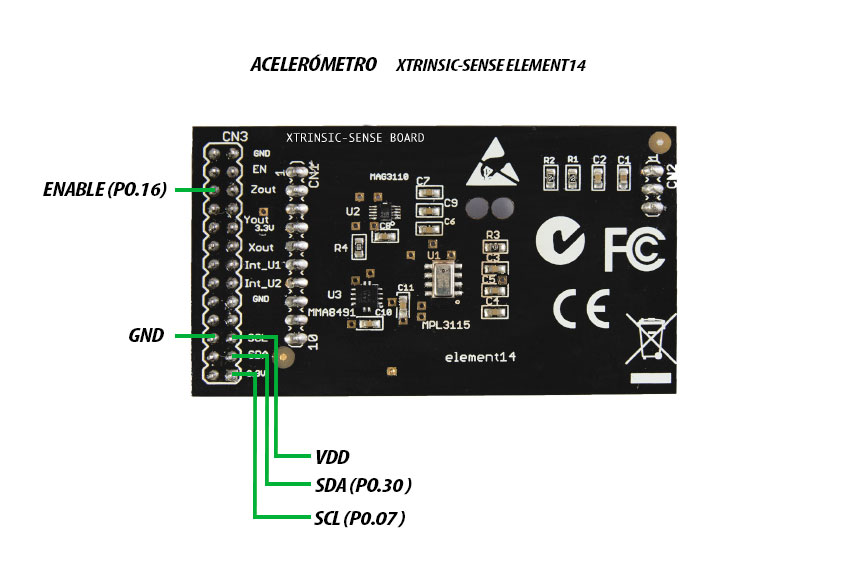
\includegraphics[scale=0.6]{figures/estructura_xtrinsic.jpg} % TODO hacer que esto no quede horrible
    \caption[Cableado del acelerómetro por I2C]{Cableado del acelerómetro por I2C}
   	\label{figuraXtrinsic}
\end{figure}

\subsection{Lectura de datos}
\label{makereference5.1.1}

El acelerómetro MMA8491Q tiene 7 registros donde se guardan los datos de acelerometría que han sido recogidos en la lectura. El primer registro es un registro de estado en el que se indica si alguno de los ejes ha cambiado desde la última muestra, los 6 registros siguientes dividen cada eje en los 8 bits más significativos y los 6 menos significativos, haciendo un total de 14 bits por eje. En la tabla que se muestra en la Figura~\ref{figuraRegistrosAcc} se puede observar la información de los 7 registros.

\begin{figure}[h]%t=top, b=bottom, h=here
	\centering
    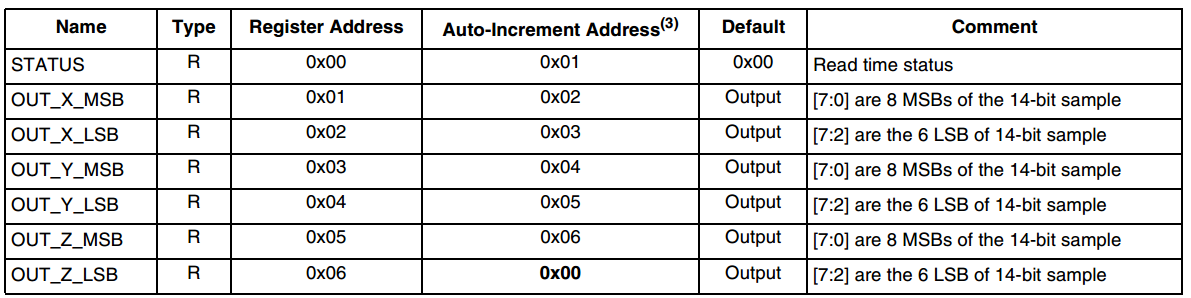
\includegraphics[width=\textwidth]{figures/registros_Acelerometro.png} % TODO hacer que esto no quede horrible
    \caption[Registros del acelerómetro]{Tabla con los registros del acelerómetro~\cite{DatasheetAcc}}
   	\label{figuraRegistrosAcc}
\end{figure}

Estos 14 bits se utilizan para especificar los valores de cada eje en un rango de +8000 mg a -8000 mg. Para ello utilizan el formato de la tabla que se puede ver en la Figura~\ref{figuraValoresAcc} sacada del datasheet~\cite{DatasheetAcc}. Se puede observar que se utiliza un Complemento a 2 para definir los números negativos. La forma de parsearlos se explicará más adelante.

\begin{figure}[h]%t=top, b=bottom, h=here
	\centering
    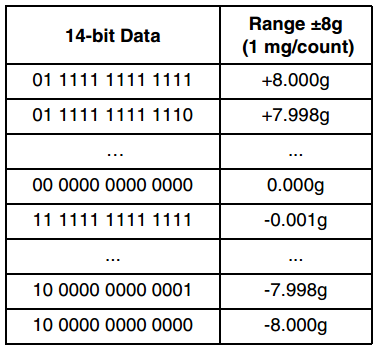
\includegraphics[scale=0.6]{figures/rango_datos_acelerometro.png} % TODO hacer que esto no quede horrible
    \caption[Rango de datos del acelerómetro]{Rango de datos del acelerómetro~\cite{DatasheetAcc}}
   	\label{figuraValoresAcc}
\end{figure}

El acelerómetro establece una serie de pasos para poder establecer la comunicación por I2C en el modo \textit{Multiple Byte Read}, que apunta al siguiente registro una vez concluida la lectura del anterior:

\begin{itemize}
	\item Se manda el comando Start condition con la dirección 0x55 y 1 bit de lectura-escritura a 0 para indicar escritura, el esclavo responde con una trama ACK.
	\item Se transmite la dirección del registro que se quiere leer y el esclavo manda una trama ACK.
	\item Se transmite el comando Repeated Start Condition con la dirección del acelerómetro, y esta vez el bit de lectura-escritura a 1 indicando lectura.
	\item El esclavo manda una trama ACK y transmite los datos del registro indicado.
	\item Por último, se transmite una trama ACK y una señal de stop para finalizar.
\end{itemize}

Una vez recibidos estos datos en la placa de Nordic, se juntan y se parsean siguiendo la siguiente fórmula:

\begin{lstlisting}[frame=single]

	WORD = (MSB << 6) | (LSB >> 2);
	
	if (WORD >= 0x2000)
		WORD -= 0x4000;

	NATURAL = (1000 * WORD + 512) >> 10;

\end{lstlisting}

Donde MSB es el byte con los bits más signigicativos, LSB es el byte con los bits menos significativos, y WORD y NATURAL son variables enteras. Durante estos pasos se amplían los 14 bits a 16 para poder dividirlos en 2 bytes y así poder enviarlos mediante Bluetooth.

\subsection{Filtrado}
\label{makereference5.4.2}

En un entorno ideal, los datos que recoja el acelerómetro en un período en el que se encuentre estático deberían ser únicamente el valor de la gravedad (1g) repartido entre los 3 ejes, ya que es una aceleración constante que experimenta cualquier objeto en este planeta.

Lejos de ese caso, la información que recibimos varía ligeramente, normalmente en una escala de unos pocos mg. Para eliminar este ruido realizamos un filtrado consistente en recoger una muestra de 10 valores e insertarlos en un Búfer circular para poder filtrarlos a través de una media ponderada. El dar pesos a los datos permite que los últimos valores no se pierdan y que la media se actualice lo suficientemente rápido en caso de cambios bruscos.

\section{Comunicación Bluetooth}
\label{makereference5.2}

Como mencionábamos en el Capítulo~\ref{makereference2}, hemos elegido el Modo de Conexión para realizar el enlace y el intercambio de datos entre la placa de Nordic y el dispositivo móvil. En este caso tendremos los roles GAP y GATT (Explicados en las Secciones~\ref{makereference2.3.2} y~\ref{makereference2.4.1}, respectivamente) que se muestran en la Tabla~\ref{tablaRoles5}. 

El dispositivo móvil actúa como Central, ya que realiza el escaneo y la conexión, y como Cliente porque es el que envía las peticiones para recibir la información.

La placa nRF51-DK actúa como Periférico, pues manda paquetes de anuncio y acepta las conexiones entrantes, y como Servidor, al ser el que guarda la información y responde a las peticiones.

\begin{table}
	\begin{center}
	\begin{tabular}[c]{|c|c|c|}
        \hline
        & GAP & GATT \\
        \hline
        Dispositivo Móvil & Central & Cliente \\
    	\hline
    	Placa nRF51-DK & Periférico & Servidor \\
    	\hline
	\end{tabular}
    \caption{Roles GAP y GATT del dispositivo móvil y de la placa nRF51-DK}
    \label{tablaRoles5}
   \end{center}
\end{table}

Empezamos configurando el Perfil de Acceso Genérico (GAP) para establecer la información que incluyen los paquetes de anuncio:

\begin{itemize}
	\item El dispositivo es sólo BLE y no utiliza Bluetooth clásico
	\item Se le permite a otros dispositivos su descubrimiento
	\item La lista de servicios que contiene, en la que aparecerá el servicio mencionado anteriormente
	\item El nombre del dispositivo, dado por una cadena de caracteres
	\item El método de conexión
\end{itemize}

Toda esta información estará disponible para cualquier dispositivo que se encuentre escaneando.\\

Seguidamente configuramos el Perfil de Atributo Genérico (GATT). Definimos el dispositivo como servidor GATT y, para encapsular los datos del acelerómetro, creamos un servicio con UUID 0xA000, al que le asignaremos una característica con UUID 0xA001. Esto se hace mediante las clases \textit{GattService} y \textit{GattCharacteristic} que nos ofrece la API de mbed. Estas clases permiten establecer los siguientes parámetros:

\textbf{Característica.} Le podemos definir un tamaño máximo y mínimo de los datos que van a contener, en nuestro caso siempre va a tener 6 bytes (3 ejes divididos en 2 bytes cada uno). También especificamos aquí que este valor es de sólo lectura.

\textbf{Servicio.} Le asignamos una lista en la que únicamente aparecerá nuestra característica.\\

Como se ha explicado en la Sección~\ref{makereference5.1.1}, los datos extraídos del acelerómetro se guardan en la nRF51-DK en tres variables de 16 bits, aunque la API BLE de mbed obliga a actualizar el valor de una característica utilizando un array de variables de 8 bits, por lo que necesitamos dividir los 16 bits de cada eje en dos bytes separados. Esto hace que el dispositivo móvil reciba la información también de este modo, por lo que se tienen que juntar de nuevo al recibirlos.


% +-------------------------------------------------------------------------+
% | References                                                              |
% +-------------------------------------------------------------------------+

% +-------------------------------------------------------------------------+
% | In order for WinEDT to index references correctly, it has to know where |
% | the file resides.  The following command is prefaced by %, and will be  |
% | ignored completely by LaTeX.  However, WinEDT will use this line to     |
% | access the external .bib bibliography file.  Also note that WinEDT can  |
% | read file path names with either "\" or "/" - LaTeX, however, doesn't   |
% | like "\", so it's easier to store a path name in the "Unix" style.      |
% +-------------------------------------------------------------------------+

%Included for Gather Purpose only.  Do NOT uncomment:
%input "references.bib"

% +--------------------------------------------------------------------+
% | This template uses the BibTeX program to format references.  The
% | 3 lines below create a separate Bibliography section and add
% | an entry for "Bibliography" to the Table of Contents.  The actual
% | data for your references (author, title, journal, date, etc.) are
% | entered in the references.bib file.  See that file for information
% | on how to enter references.
% +--------------------------------------------------------------------+

\bibdata{references}
\bibliography{references}
\addcontentsline{toc}{chapter}{Bibliography}

% +--------------------------------------------------------------------+
% | Finally, we generate the appendix.  To add or delete appendices,
% | add or remove the line
% |
% |     \input{appendixX.tex}
% |
% | where "X" is the letter designation of the Appendix (A, B, C, etc.)
% | You should have one \input{appendixX.tex} line and a corresponding
% | file appendixX.tex for each appendix.                                 |
% +--------------------------------------------------------------------+

\appendix
% +--------------------------------------------------------------------+
% | Appendix A Page (Optional)                                         |
% +--------------------------------------------------------------------+

\cleardoublepage

\chapter{Title for This Appendix}
\label{Appendix:Key1}


% +--------------------------------------------------------------------+
% | Enter text for your Appendix page in the space below this box.     |
% |                                                                    |
% +--------------------------------------------------------------------+

% +--------------------------------------------------------------------+
% | Appendix B Page (Optional)                                         |
% +--------------------------------------------------------------------+

\cleardoublepage

\chapter{Title for This Appendix}
\label{Appendix:Key2}

% +--------------------------------------------------------------------+
% | Enter text for your Appendix page in the space below this box.     |
% |                                                                    |
% +--------------------------------------------------------------------+


\end{document}
